% Ce fichier main.tex est le fichier principal \`{a} partir duquel tout est g\'{e}n\'{e}r\'{e}
% This file is the main file where the final document is generated
\documentclass{these-dbl}

% Remplir les metadonnees du pdf
% Fill the pdf metadata
\hypersetup{
%    pdfauthor   = {XYZ},
%    pdftitle    = {Th\`{e}se de doctorat de XYZ},
%    pdfsubject  = {Th\`{e}se de doctorat de XYZ},
%    pdfkeywords = {mots-cl\'{e}s},
}

\geometry{vmargin=4.0cm}

% Spécifier vos fichiers de bibliographie
% Specify you bibliography files here
\addbibresource{./biblio.bib}

\providecommand{\tightlist}{%
  \setlength{\itemsep}{0pt}\setlength{\parskip}{0pt}}

\begin{document}
\pagenumbering{gobble}
% Page de garde avec commande \maketitle
% Front cover calling \maketitle
\input{./00-Couverture-these/pagedegarde}

% Sélectionner la langue du contenu suivant cette ligne
% Select the content language following this line
\selectlanguage{french}

% Inclusion du chapitre remerciement
% Input acknowledgement chapter
\clearemptydoublepage
\begin{refsection}

\hypertarget{remerciements}{%
\chapter*{Remerciements}\label{remerciements}}

Il y a un peu plus de vingt ans, qui aurait pu imaginer que le petit
garçon que j'étais, blotti dans sa serviette de plage, terrifié à la
seule pensée de fouler ce sable répugnant, souillé par les laisses de
mer et infesté de ces immondes amphipodes bondissant de toute part, se
destinerait à rédiger une thèse en écologie marine ? Ces quelques lignes
ne pourront exprimer toute la gratitude que j'ai envers vous, vous qui
m'avez permis d'arriver jusqu'au bout de ce périple.

Je souhaite tout d'abord exprimer ma sincère gratitude à Sakina-Dorothée
Ayata, Emmanuelle Cam, Thibaut de Bettignies d'avoir accepté de faire
partie de ce jury de thèse. Je souhaite remercier tout particulièrement
Stéphane Dray et David Mouillot pour avoir accepté d'en être les
rapporteurs.

Je remercie également Anik Brind'Amour, Philippe Cugier, Clément Garcia
Cédric Gaucherel, Olivier Gauthier pour avoir eu la gentillesse de faire
partie de mon CSI. Merci infiniment pour votre temps et votre écoute
attentive. Merci pour vos conseils tout au long de cette thèse, qui en
ont grandement amélioré la qualité.

Merci à Stanislas Dubois d'avoir dirigé cette thèse et pour l'écoute et
tout le temps que tu m'as accordé durant toute cette thèse.

Je souhaite exprimer ma profonde gratitude à mes directeurs de thèse,
débutant par toi, Martin, pour avoir accepté de m'accueillir sous ton
aile bienveillante dès le Master. Mes remerciements s'étendent également
à Aurélien et Mathieu pour leur participation essentielle dans cette
formidable aventure qu'a constituée l'encadrement de ma thèse. Votre
curiosité intellectuelle insatiable et votre rigueur m'ont constamment
poussé vers l'excellence, enrichissant indéniablement mon parcours. La
gentillesse et la bienveillance que vous avez tous trois manifestées à
mon égard ont grandement contribué au plaisir que j'éprouvais à me
rendre au laboratoire chaque jour.

Je tiens à exprimer ma profonde gratitude à tous ceux qui ont contribué
et qui contribuent encore au programme de suivi REBENT. Sans votre
travail assidu et votre dévouement, cette thèse n'aurait pas vu le jour.
I would also like to extend heartfelt thanks to Graham Edgar, Lizzi Oh,
and Rick Stuart-Smith for your invaluable assistance throughout my PhD
journey. Your dedication, alongside the tremendous efforts of all the
volunteers involved in the Reef Life Survey Program, has been
instrumental in the progression and success of my research. Your
contributions have not only enriched my work but also underscored the
profound impact of collaborative endeavour.

Je tiens à exprimer toute ma reconnaissance à Olivier Gauthier et
Emmanuelle Cam qui m'ont généreusement donné l'opportunité d'enseigner
durant ces trois années. Chaque heure passée en compagnie des étudiants
a été pour moi une source de joie intense, me poussant à approfondir
avec rigueur les sujets que j'avais la responsabilité de leur
transmettre.

Ma passion pour l'enseignement, je la dois en grande partie à toi,
Olivier. Tes cours n'ont pas été seulement instructifs ; ils ont été une
véritable révélation. Cependant, cette vocation ne s'est pas nourrie de
ta seule influence, aussi significative soit-elle (et c'est bien dommage
!). Je suis également redevable à Gauthier Schaal et Jacques Grall, qui
m'ont montré qu'enseigner pouvait se faire dans une ambiance chaleureuse
et décontractée. Enfin, mes sincères remerciements vont à Christophe et
David. Votre approche innovante et particulière de l'enseignement a
profondément transformé ma conception de la pédagogie, et pour cela, ma
gratitude est infinie.

Je souhaite du plus profond de mon coeur remercier Emilien, Touria,
Aline B., Aurélien B., Antoine, Mathieu, Céline, Philippe, Amelia,
Gabin, Stan, Justine, Aline G., Pierre-Olivier, Martin, Flavia, Aurélien
T. et Mick' pour faire du LEBCO et de sa salle de pause un endroit si
chaleureux, merci infiniment pour ces fous rires.

Un immense merci à Véronique pour avoir aidé durant ces trois années à
naviguer dans les différents arcanes administratifs d'Ifremer et de
m'avoir aidé à préparé mes différentes missions.

Un énorme merci à tous les doctorants (et les pièces rapportées !) de
l'Open Space pour cette ambiance incroyable qui nous booste chaque jour
! Une pensée spéciale pour ceux qui ont déjà pris leur envol vers de
nouvelles aventures : Bastien, Kévin, Lyndsay, Marion, Lou, et Alex.
Léa, dont la gentillesse et le rire ont le pouvoir magique de réchauffer
l'Open Space, même lors des matinées frisquettes d'automne, d'hiver, de
printemps ou d'été. Un p'tit clin d'oeil à notre Dinde Supérieure,
Laure, doyenne incontestée de notre petit univers ; chacune de nos
discussions a été un vrai kif ! Et toi, Mathisse, tu es simplement la
meilleure (et pas seulement pour le café brûlant qui m'accueille chaque
matin). Impossible de résumer ici tous ces moments épiques vécus
ensemble, que ce soit en installant du carrelage et des moulures dans le
bureau de Mathieu, lors des sessions cours de surf ou lors de nos
innombrables soirées bars. En parlant bar toi, Bastouille, avec tes
exploits légendaires, tu restes indétrônable ! Nos disucssions Tour de
France et les étapes dans le Pays-Basque resteront gravés dans ma
mémoire. Un immense merci également, pour ces moments ``oxygénation''
ces dernières semaines, j'en avais grandement besoin. Mathieu, tu es
sans conteste LA `pièce rapportée' de cet Open Space, merci pour ces
discussions et ces fous rires en pause ou à la cantine qui resteront
gravés dans ma mémoire ! Chonchon, un merci tout spécial pour ton super
boulot durant ton M2, essentiel pour ma thèse, et merci pour tous ces
mèmes politiques croustillants sur Twitter, quelle rigolade ! Merci,
Irene, d'avoir enduré mon espagnol hésitant sans jamais perdre patience,
c'est un exploit ! Quant aux petits nouveaux, Lucas, Maeva, et Chloé,
votre aventure ne fait que commencer, mais je suis déjà ravi d'avoir
croisé votre route. Je suis persuadé que vous allez faire un excellent
job. Savourez chaque instant, malgré les défis que la thèse représente,
ça en vaut la peine ! Un immense merci à tous pour ces moments
inoubliables !

Un phénoménal big-up à mon crew, la team ``A Fond la Fonte'' : Manon,
Marine, Thomas, Mathisse, Laure, Aurélien, Mathieu ! J'avoue, mon
assiduité brillait peut-être plus à la cantine qu'à la salle de sport.
Mais qu'importe, chaque déjeuner passé ensemble était épique. Merci pour
ces instants mémorables !

Je tiens à saisir cette opportunité pour exprimer ma profonde gratitude
envers tous mes amis qui ont jalonné mon parcours depuis mon arrivée à
Brest. Un merci tout particulier à Elodie, Elodie, Pierre, Thibault,
François, Anthony, Mathilde, Angelina, Maurane, Christophe et David pour
tous ces précieux moments partagés. Ma reconnaissance s'étend également
aux amis rencontrés au cours de ce voyage académique, notamment Lyndsay,
Léa, Lou, Kévin, Lucas, Pierre-Léo, Aurélien, Gabin, Mathieu et Noémie,
Romain, Fred, Gaspard et Claire, qui ont chacun illuminé ce voyage.

Merci au Tortuga, aux Fauvettes et maintenant à Gourmand, Mais Pas Que
(a.k.a. l'After Work) d'avoir été les partenaires officiels de ma thèse.

Je souhaite rendre un hommage tout particulier à Masha, mon tigre
domestique, qui a fait de moi son humain de compagnie.

Merci infiniment à ma famille, et surtout à mes parents, vous méritez
amplement toute ma gratitude pour votre soutien constant tout au long de
mes études, une fondation solide qui m'a porté jusqu'à cet instant où je
rédige ces quelques phrases. Sans vous, rien de tout cela n'aurait été
possible et je vous en suis infiniment reconnaissant. Une petite mention
spéciale à toi Guillaume, pour avoir partagé ces années inoubliables à
Brest avec moi, affichant avec fierté les couleurs du Stade Brestois 29.
Ensemble, nous avons bravé la pluie, le vent, la neige, ou même les
trois à la fois, dans l'arène légendaire du stade Francis-Le Blé. Merci
frangin !

Je souhaite également remercier ma belle famille. Gilles, Dominique,
Gwen (sans oublier le p'tit Maël), un merci du fond du cœur pour votre
accueil chaleureux, ainsi que pour le soutien indéfectible et
l'affection que vous m'avez généreusement offerte au fil des années.

Gaëlle, ton amour et ton soutien inconditionnel ont été mon refuge et ma
force durant cette thèse. Ces années n'auraient pas eu la même saveur
sans ta présence constante et rassurante à mes côtés. Je sais que les
derniers mois ont été rudes pour toi. Sans toi, ce travail de thèse
n'aurait pas seulement été plus difficile --- il aurait été impossible.
Je t'aime.

Ces remerciements sont déjà beaucoup trop longs, mais sache que je te
remercie du font du coeur toi, toi que je n'ai malheureusement pas eu la
place de citer, mais qui a croisé ma route pendant cette aventure
universitaire et l'a rendu unique. Merci infiniment.

\printbibliography[heading=subbibintoc, title={Bibliographie}]
\end{refsection}

\clearemptydoublepage
% Ne pas oublier cette commande qui g\'{e}n\`{e}re la page de couverture avant
% This command will generate the front cover
\frontmatter
% \renewcommand{\contentsname}{Table of Contents}
\tableofcontents %sommaire %table of content
\listoffigures
\listoftables
%\shorttableofcontents{Sommaire}{0}

\clearemptydoublepage
\mainmatter

\hypertarget{introduction}{%
\chapter*{Introduction}\label{introduction}}
\addcontentsline{toc}{chapter}{Introduction}

\chaptermark{Introduction}

\hypertarget{les-uxe9costysuxe8mes-cuxf4tiers}{%
\section*{Les écostysèmes
côtiers}\label{les-uxe9costysuxe8mes-cuxf4tiers}}
\addcontentsline{toc}{section}{Les écostysèmes côtiers}

La notion d'habitat est essentielle en écologie. Cette notion englobe
non seulement le lieu où une espèce peut être trouvée, le(s) lieu(x) où
elle réalise son cycle de vie, mais également l'ensemble des conditions
abiotiques et biotiques qui permettent le maintien de sa population
\autocite{Hall_1997}. Certaines espèces animales ou végétales ont la
capacité de modifier leur environnement de nombreuses façons
différentes, comme en modifiant les conditions environnementales
\autocite{Ellison_2019} ou en produisant des structures
tridimensionnelles complexes permettant d'abriter d'autres espèces
\autocite{Darling_2017}. Ces espèces sont qualifiées d'espèces
ingénieurs \autocite{Jones_1996}. Ces espèces ingénieurs peuvent de par
leur seule présence caractériser un habitat, c'est pourquoi dans la
suite de ce manuscrit, nous allons qualifier les habitats créés par ces
espèces d'habitats biogéniques.

Les habitats biogéniques structurent la dynamique des écosystèmes
benthiques côtiers auxquels elles sont associées \autocites[
]{Duffy_2006}{Teagle_2017}. Ces habitats vont promouvoir une plus grande
diversité spécifique au sein des écosystèmes qui les abritent
\autocites[ ]{Romero_2015}{Sunday_2016}, notamment de par leur capacité
à tamponner les conditions environnementales locales en modifiant par
exemple la température \autocite{Bulleri_2018}. A une échelle locale,
les habitats biogéniques tendent donc à augmenter l'hétérogénéité
spatiale de l'environnement et par conséquent augmentent la diversité et
l'abondance de niches environnementales disponibles pour d'autres
espèces \autocites[ ]{Duffy_2006}{Hewitt_2005}. Ces modifications
locales de l'environnement par les habitats biogéniques entretiennent
des boucles de rétroactions négatives \autocite{Kefi_2016}, ces boucles
de rétroactions négatives ont des effets stabilisateurs des conditions
environnementales, ce qui à une échelle globale augmente la résilience
des écosystèmes face aux perturbations entraînées par le changement
climatique global (fig.~\ref{fig:1}; \textcite{Bulleri_2018} ;
\textcite{Jurgens_2022}). Un exemple simplifié est celui des herbiers
marins, qui assurent la protection des mezobrouteur\footnote{Les
  mezobrouteurs sont de petits invertébrés herbivores d'une taille
  inférieure ou égale à 2,5 cm \autocite{Beermann_2018}.} contre leurs
prédateurs, qui vont se nourrir des épiphytes permettant à l'herbier de
se maintenir et de s'agrandir. Ainsi, ces boucles de rétroactions
négatives ont des effets stabilisateurs des conditions
environnementales, ce qui à une échelle globale augmente la résilience
des écosystèmes face aux perturbations entraînées par le changement
climatique global \autocites[ ]{Bulleri_2018}{Jurgens_2022}.

La promotion de la biodiversité par les habitats biogéniques a également
un impact sur les services écosystémiques fournis par les écosystèmes
marins. Ces habitats biogéniques sont notamment des zones importantes
pour le cycle de vie de poissons à forte valeur commerciale. Par
exemple, les prés-salés et les herbiers marins sont des zones de
nourricerie essentielles au développement des juvéniles comme ceux du
bar commun (\emph{Dicentrarchus labrax}) \autocites[
]{Stamp_2022}{Maxwell_2017}. Ces habitats biogéniques ont également un
fort impact économique ; les récifs coralliens supportent par exemple
une industrie du tourisme conséquente (valeur estimée à près de
36~milliards de dollars par an ; \textcite{Spalding_2017}). Enfin, les
habitats biogéniques jouent un rôle particulièrement important dans la
lutte contre l'érosion, via leur effet de stabilisation du sédiment
\autocite{Reidenbach_2018} ou bien en réduisant l'énergie des vagues
lors d'évènements extrêmes comme les tempêtes \autocite{Krauss_2019} ou
bien les tsunamis \autocite{Alongi_2008}.

Malgré leur importance, les écosystèmes côtiers font face à de
nombreuses menaces comme l'acidification des océans
\autocite{Doney_2009}, l'augmentation des températures
\autocite{IPCC_2021_technical_summary}, l'augmentation du nombre et de
la fréquence des évènements climatiques extrêmes \autocite{Oliver_2018},
ainsi que de leur surexploitation \autocites[ ]{Lotze_2006}{Lotze_2009}.
Ainsi, les habitats biogéniques qui sont de nature souvent fragile, car
formés par des espèces souvent sensibles aux différents impacts
anthropiquesont et ont décliné tant en qualité (i.e.~dégradation de
l'état écologique, ou perte de complexité, etc.), qu'en quantité
(i.e.~souvent exprimé comme une réduction de leur superficie) à travers
l'Europe et dans le monde entier \autocites[ ]{Airoldi_2007}[
]{Dunic_2021}[ ]{McCauley_2015}{Waycott_2009}. Ces pertes des habitats
biogéniques sont l'un des principaux moteurs du déclin de la
biodiversité auquel nous assistons actuellement \autocites[
]{Airoldi_2007}[ ]{ipbes_2019}{McCauley_2015}.

Ces différentes pressions d'origine anthropique et leurs conséquences
sur les habitats biogéniques vont affecter par effet de cascade
fonctionnement et dynamique globale des écosystèmes côtiers \autocites[
]{Rocha_2015a}[ ]{Sara_2021}{Wernberg_2016}. Les écosystèmes étant des
objets dynamiques, ils peuvent répondre de différente manière à ces
pressions. Après avoir dépassé leur seuil de résistance envers ces
perturbations, ils vont être transformés de façon linéaire, ou bien de
manière non linéaire. Ces changements non linéaires entraînent des
modifications profondes des écosystèmes appelés ``changement de régime''
\autocite{Scheffer_2001}. Dans le cas des transitions linéaires, il
serait possible d'identifier des états d'habitats différents de l'état
pristin plus ou moins dégradé \autocite{Spake_2022}. Lorsque les
transformations suivent des tendances non linéaires, l'apparition de
seuils empêchera le retour à l'état pristin des écosystèmes
\autocite{Spake_2022}.

Ces changements de régimes et d'états ont d'ores et déjà été observés à
travers un grand nombre d'écosystèmes terrestres et marins, par exemple
: la transition entre la toundra et la forêt boréale
\autocite{Folke_2004}, entre la forêt et la savane \autocites[
]{Debra_2004}{Folke_2004}, mais également, comme pour les forêts de
laminaires qui peuvent laisser place à des déserts d'oursins \autocites[
]{Carnell_2020}{Rogers-Bennett_2019}, ou bien encore les récifs
coralliens supplantés par des macroalgues \autocites[
]{Folke_2004}{OBrien_2018}. Le déclin des habitats biogénique est
notamment l'un des moteurs des changements de régimes observés ces
dernières décennies \autocites[ ]{Rocha_2015a}{Wernberg_2016}.

Pour éviter la dégradation des écosystèmes marins liée à la disparition
des habitats biogéniques, les écologues font face à de nombreux défis à
relever. Un premier défi consiste à identifier et décrire les différents
types d'habitats biogéniques à l'échelle mondiale de façon adéquate pour
identifier les changements d'état d'habitat. En effet, les typologies
existantes ont du mal à détecter ces changements \autocite{Cooper_2019},
ce qui entrave la mise en place de mesures de gestion efficaces
\autocite{Ware_2020}. Par conséquent, il est essentiel de développer une
typologie d'habitat mondiale basée sur les suivis biologiques existants
\autocite{Cooper_2019} afin de mieux coordonner les politiques de
préservation des habitats côtiers \autocite{Ware_2020}. Le second défi
réside dans la prévention des changements d'état d'habitats biogéniques.
Pour ce faire, il est nécessaire d'identifier les facteurs externes et
internes qui contribuent d'une part à leur résilience et d'autre part
qui facilitent les transitions vers d'autres types d'habitats. Grâce à
une meilleure connaissance de ces facteurs, il sera possible
d'identifier des zones géographiques plus à risque de changement de
régime, et donc de mettre en place des mesures de suivi adéquat
permettant de réagir dès les premiers signes de changement de régime
observés.

Le développement de nouveaux outils méthodologiques de modélisation peut
permettre de faire face au premier défi. Pour le second, deux approches
différentes existent : une expérimentale, grâce à des expérimentations
\emph{in situ} ou en méscosome et une approche de modélisation. Ces
expérimentations \emph{in situ} ou en mésocosme présentent certains
avantages comme celui d'avoir une observation directe des phénomènes
étudiés \autocite{Fulton_2019}. Cependant, elles sont souvent réalisées
à des échelles spatiales restreintes et sur des périodes de temps
limitées, particulièrement lorsque les études s'intéressent aux
écosystèmes marins du fait de leurs contraintes \autocite{Witman_2015}.
Ainsi, les interactions entre les organismes, les conditions
environnementales et les pressions observées lors de ces
expérimentations peuvent être différentes de ce qui passe à plus large
échelle spatiale et/ou temporelle. Les résultats de ces expérimentations
peuvent alors être plus difficilement généralisables
\autocite{Witman_2015}.

Pour surmonter ces contraintes, l'utilisation d'outils de modélisation
peut se révéler utile. Les modèles sont des représentations simplifiées
des systèmes écologiques qui permettent leur étude à des échelles
spatiotemporelles plus grandes. Les modèles en écologie peuvent être
regroupés en deux catégories : de manière mécanistique ou corrélatives
\autocite{Kearney_2010}. Ces modèles peuvent être complexifiés à loisir
selon les hypothèses de recherche pour mieux prendre en compte la
complexité réelle des écosystèmes \autocite{Cartwright_2016}. Les
modèles permettent également de prédire les changements futurs des
habitats biogéniques en fonction des scénarios de changement climatique
\autocite{Curd_2023}.

L'objectif principal de cette thèse est d'améliorer la compréhension et
la prévision des changements potentiels dans les habitats biogéniques
des environnements benthiques côtiers. Pour cela, elle se concentre sur
l'identification des types d'habitats benthiques, l'exploration de leurs
états alternatifs et l'analyse des facteurs favorisant l'établissement
de ces différents états. Afin d'atteindre cet objectif, la thèse
s'appuie sur les données collectées par le programme \emph{Reef Life
Survey}, qui a effectué depuis 2008 des suivis des habitats et de la
faune des récifs côtiers à travers le monde. Grâce à ces données, la
thèse vise à identifier les principaux types d'habitats benthiques
côtiers en développant de nouvelles méthodes pouvant être adaptées à
d'autres écosystèmes. Elle contribue également à acquérir de nouvelles
connaissances sur les facteurs environnementaux et les pressions
d'origine humaine qui influent sur le maintien ou le changement de ces
habitats biogéniques.

Ce travail de thèse est découpé en trois axes majeurs qui s'attèlent à
répondre à ces différentes questions.

\begin{enumerate}
\def\labelenumi{\arabic{enumi}.}
\tightlist
\item
  Définition d'une typologie d'habitats côtiers à l'échelle du globe à
  partir des données \emph{in situ} issues du programme \emph{Reef Life
  Survey}.
\end{enumerate}

Le but de cet axe est de développer une méthodologie d'identification de
typologie d'habitat à partir de données de substrat fournies par le
programme de suivis des communautés de récifs \emph{Reef Life Survey}
\autocite{Edgar_2004}.

Le \emph{Reef Life Survey} recense grâce à des plongeurs les poissons
nageant en pleine eau, au niveau du récif sur un transect de 50m de long
et de 10m de large. Puis, un second passage est effectué le long du
transect pour dénombrer la faune cryptique et benthique associée au
récif. Pour cette seconde passe, la largeur du transect est réduite à 4m
(fig.~\ref{fig:2}). Enfin, lors d'un troisième passage, 20 quadrats sont
photographiés tous les 2,5m \autocite{Edgar_2020}. Les pourcentages de
couverture de faune et flore benthique sont ensuite évalués visuellement
grâce à l'outil d'annotation d'image \emph{Squidle+}
(\url{https://squidle.org/}).

Une nouvelle méthodologie de groupement adaptée à ces données a été
développée pour créer une typologie des habitats benthiques. Elle est
présentée, justifiée en détail dans l'Annexe A et sera bientôt envoyée à
une revue.

\begin{enumerate}
\def\labelenumi{\arabic{enumi}.}
\setcounter{enumi}{1}
\tightlist
\item
  Distribution des habitats côtiers \& identification des zones à risque
  de changements de types d'habitats
\end{enumerate}

La seconde partie de cette thèse s'intéressera à modéliser les niches
environnementales de chacun des types d'habitats précédemment découverts
pour (1) identifier les seuils environnementaux qui favorisent
l'occurrence de ces habitats (2) identifier les zones capables d'abriter
plusieurs types d'habitats (3) définir des habitats alternatifs en
étudiant le chevauchement de leurs niches environnementales. Un stage de
M2 a déjà été encadré sur cette thématique pour réaliser une première
exploration de ces questions de recherche.

L'un des sujets de discussion que le doctorant souhaite aborder lors de
ce CSI concerne l'identification d'une stratégie de modélisation
efficace pour répondre aux questions de recherche pendant la période
restante de son contrat de thèse.

\begin{enumerate}
\def\labelenumi{\arabic{enumi}.}
\setcounter{enumi}{2}
\tightlist
\item
  Potentiel des \emph{jSDM} pour l'étude des impacts des changements
  d'habitats sur les communautés : une perspective préliminaire
\end{enumerate}

Les habitats biogéniques jouent un rôle crucial dans les écosystèmes
côtiers en façonnant les communautés animales. Les perturbations
d'origine humaine perturbent l'état écologique de ces habitats et ont un
impact significatif sur les communautés associées en modifiant à la fois
les habitats des espèces et les conditions environnementales. La
présence d'une espèce dans un lieu et à un moment donné est limitée par
les conditions environnementales et les interactions avec d'autres
espèces, qui forment collectivement la niche environnementale de
l'espèce au sein de la communauté. Pour comprendre et anticiper les
conséquences des modifications de l'habitat sur le fonctionnement des
écosystèmes, il est essentiel de mener des études détaillées sur les
niches environnementales des espèces, englobant les facteurs abiotiques
et biotiques, ainsi que l'effet de l'habitat.

Cependant, en raison de la forte interdépendance entre l'habitat,
l'environnement et les interactions entre espèces dictées par la niche
environnementale, la compréhension des conséquences de la modification
de l'habitat nécessite de démêler les effets individuels de chaque
facteur. Des outils de modélisation prometteurs, tels que les modèles de
distribution d'espèces conjointe (\emph{Joint Species Distribution
Models} ou \emph{jSDM}), sont récemment apparus comme des solutions
potentielles à ce défi. Néanmoins, il y a actuellement un manque de
recul pour mettre en oeuvre de manière efficiente ces outils complexes
et exigeants, notamment en ce qui concerne leurs capacités explicatives
et prédictives, ainsi que leurs possibilités d'interprétation. C'est
pourquoi, avant de pouvoir être déployé sur un cas d'étude complexe, il
est nécessaire de comprendre le comportement de ces outils sur un jeu de
données connu pour évaluer l'impact des choix de modélisation sur les
performances d'un \emph{jSDM}. Ce travail a fait l'objet d'une
publication soumise au journal \emph{Methods in Ecology and Evolution}.
L'article soumis est présenté dans l'Annexe C.


\printbibliography[heading=subbibintoc, title={Bibliographie}]
\clearemptydoublepage

\begin{refsection}

\hypertarget{essential-ingredients-in-joint-species-distribution-models}{%
\chapter{Essential ingredients in Joint Species Distribution
Models}\label{essential-ingredients-in-joint-species-distribution-models}}

\hypertarget{preambule-chapter1}{%
\section*{Préambule}\label{preambule-chapter1}}
\addcontentsline{toc}{section}{Préambule}

Les modèles de distribution d'espèces (\emph{Species Distribution
Models}, \emph{SDM}) ont récemment bénéficié d'avancées méthodologiques
significatives, en particulier grâce à l'adoption de modèles
statistiques multivariés, désignés sous le terme de \emph{jSDM}
(\emph{Joint Species Distribution Models}; \textcite{Warton_2015}). Ces
modèles se révèlent prometteurs pour élucider de nombreuses questions en
écologie des communautés. Ils permettent de comprendre l'effet de
l'environnement, des traits fonctionnels, de l'histoire évolutive sur
les espèces étudiées, les raisons leur présence dans une zone donnée, et
enfin la structure de la communauté étudiée \autocites[
]{Warton_2015}{Ovaskainen_2017a}. Ces méthodologies ont suscité un
intérêt croissant au sein de la communauté écologique pour diverses
raisons. En premier lieu, elles semblent particulièrement adaptées pour
décrypter une multitude de processus écologiques (voir Table 1 dans
\textcite{Ovaskainen_2017a}). En second lieu, elles semblent manifester
une capacité prédictive supérieure en comparaison avec les \emph{SDM}
\autocite{Norberg_2019}, et se distinguent par leur capacité à inférer
des interactions interspécifiques \autocites[ ]{Warton_2015}[
]{Ovaskainen_2017a}{Ovaskainen_2017b}.

Néanmoins, certaines incertitudes subsistent quant à l'application
optimale de ces modèles. La flexibilité intrinsèque de ce cadre
méthodologique suscite des interrogations sur la stratégie à appliquer :
pour optimiser l'inférence des processus écologiques d'une part, et la
performance prédictive d'autre part. Des questions restent en suspens,
quant à l'inclusion par exemple, de données sur les traits fonctionnels
des espèces de la communauté étudiée, difficile à collecter, et de leur
impact sur le pouvoir explicatif et prédictif des modèles. Si leur
capacité à améliorer la précision prédictive a été largement démontrée
sur des ensembles de données de présence/absence, notamment dans les
études de \textcite{Norberg_2019} et \textcite{Wilkinson_2020}, la
performance de ces modèles quand ils sont ajustés à des données
d'abondance reste, à notre connaissance, insuffisamment explorée dans la
littérature. Certains travaux récents ont exprimé des réserves quant à
la capacité de ces méthodes à déduire efficacement les réseaux
d'interactions interspécifiques à partir de données de présence/absence
\autocites[ ]{Blanchet_2020}[ ]{Violet_2020}{Poggiato_2021}.

Il est/semble nécessaire d'évaluer la sensibilité de l'approche par
\emph{jSDM}, avant d'envisager d'utiliser ce genre de modèles pour
réaliser des inférences sur les processus écologiques et des prédictions
qui visent à déterminer l'importance des habitats biogéniques dans la
structuration des communautés benthiques en utilisant des ensembles de
données d'abondance collectées à grande échelle, par exemple celles
issues du programme \emph{Reef Life Survey} (\emph{RLS}). Cette
évaluation a été réalisée en développant une méthodologie d'évaluation
des performances des \emph{jSDMs} et en l'appliquant à un jeu de données
collectées par le programme de recherche \emph{REBENT}. Dans le cadre de
ce chapitre, nous nous sommes intéressés à un sous-ensemble du jeu de
données du \emph{REBENT}, avec un focus sur la communauté de polychètes
intertidale inféodée à deux habitats différents : les sédiments nus et
des herbiers intertidaux dont les processus écologiques ont déjà été
étudiés le long de la côte bretonne \autocites[
]{Boye_2017}{Boye_2019a}. L'objectif est de vérifier si étendre
l'approche \emph{jSDM} à une échelle globale telle que celle présentée
par le \emph{RLS} serait pertinent pour quantifier l'influence des
habitats biogéniques sur la structure des communautés faunistiques. Ceci
afin de mieux prédire et comprendre les conséquences de la disparition
des habitats biogéniques.

Ce chapitre de thèse a déjà fait l'objet d'une communication orale
``\emph{Effects of including community-level or species-specific data on
the performances of a Joint Species Distribution Model: a case study
with species-rich marine benthic communities}''. International
Statistical Ecology Conference 2022. Un préprint a été téléchargé sur la plateforme 
\emph{bioRxiv} "\emph{Essential ingredients in Joint Species Distribution Models: influence on interpretability, explanatory and predictive powe -
Clément Violet, Aurélien Boyé, Mathieu Chevalier, Olivier Gauthier, Jacques Grall, Martin P. Marzloff
bioRxiv 2022.12.19.519605; doi: https://doi.org/10.1101/2022.12.19.519605}"
Une publication a été soumise, et
envoyée en revue par deux fois en quasiment un an, au journal
\emph{Methods in Ecology and Evolution} a été récemment refusée. C'est
pourquoi ce chapitre de thèse devrait ainsi être prochainement soumis
pour publication au \emph{Journal of Applied Ecology}.

\clearpage

\hypertarget{abstract-chapter1}{%
\section{Abstract}\label{abstract-chapter1}}

\begin{enumerate}
\def\labelenumi{\arabic{enumi}.}
\item
  \emph{Joint Species Distribution Models} (\emph{jSDM}) are
  increasingly used to explain and predict biodiversity patterns.
  \emph{jSDMs} account for species co-occurrence patterns and can
  include phylogeny or functional traits to better capture the processes
  shaping communities. Yet, several factors may alter the
  interpretability and predictive ability of \emph{jSDMs} : missing
  abiotic predictors, omitting ecologically-important species, or
  increasing the number of model parameters by adding phylogeny and/or
  trait information.
\item
  We developed a novel framework to comprehensively assess the
  interpretability, explanatory and predictive power of \emph{jSDMs} at
  both species and community levels. We compared performances of four
  alternative model formulations : (1) a \emph{Bench}mark \emph{jSDM}
  with only abiotic predictors and residual co-occurrence patterns, (2)
  a \emph{jSDM} adding phylogeny to the \emph{Bench}mark, (3) a
  \emph{jSDM} adding traits to model 2, and (4) the \emph{Bench}mark
  \emph{jSDM} with additional non-target species that are not of direct
  interest but potentially interact with the target assemblage. Models
  were fitted on both presence/absence and abundance data for 99 target
  polychaete species sampled in two coastal habitats over 500km and 8
  years, along with information on 179 non-target species and traits
  data for the target species.
\item
  For both presence/absence and abundance data, explanatory power was
  good for all models but their interpretability and predictive power
  varied. Relative to the \emph{Bench}mark model, predictive errors on
  species abundances decreased by 95\% or 53\%, when including
  non-target species, or phylogeny, respectively. These differences
  across models relate to changes in both species-environment
  relationships and residual co-occurrence patterns. While considering
  trait data did not improve explanatory or predictive power, it
  facilitated interpretation of trait-mediated species response to
  environmental gradients.
\item
  This study demonstrates that any \emph{jSDM} formulation comes with
  tradeoffs between either explaining or predicting the occurrence or
  abundance of species. Hence, it highlights the need to compare
  alternative model formulations using the original and comprehensive
  assessment framework proposed in this study. Overall, this work
  contributes to a better understanding of \emph{jSDM}s' performances
  across multiple facets and provides insights and tools for model
  selection based on specific objectives and available data.
\end{enumerate}

\clearpage

\hypertarget{introduction-chapter1}{%
\section{Introduction}\label{introduction-chapter1}}

Community ecology aims at describing, explaining, and predicting changes
in communities \autocite{Tredennick_2021}. Understanding the processes
that determine species distribution is a prerequisite to characterize
and predict community structure and associated ecological dynamics,
which is critical to inform effective management or restoration measures
in a rapidly changing world \autocites[ ]{Dietze_2018}{Brudvig_2022}.
\emph{Joint Species Distribution Models} (\emph{jSDM}) are particularly
well-suited tools to address these challenges, whether to characterize
the processes that shape observed communities \autocites[
]{Warton_2015}{Ovaskainen_2017b}, or to predict future changes in
species assemblages \autocites[ ]{Norberg_2019}{Pollock_2020}.

\emph{jSDMs} are multivariate (i.e.~multi-species) extensions of
\emph{Species Distribution Models} (\emph{SDMs}), which have been
broadly applied over the past decades - across all terrestrial and
marine realms - to understand and predict both species occurrences
\autocites[ ]{Elith_2006}{Norberg_2019} and species abundances
\autocites[ ]{Howard_2014}{Waldock_2022} using a set of covariates
(e.g.~climatic variables). Relative to \emph{SDMs}, \emph{jSDMs}
explanatory power can benefit from accounting for species assembly rules
\autocite{Ovaskainen_2017a}. In particular, relative to single-species
\emph{SDMs} that only consider the abiotic niche of species (i.e.~the
Grinellian niche), \emph{jSDM} can theoretically also account for
interspecific interactions (i.e.~the Eltonian niche).

In \emph{jSDMs}, the variability in community composition not explained
by covariates is captured by a residual covariance matrix representing
species co-occurrence patterns potentially representing biotic
interactions \autocite{Ovaskainen_2017a}. This feature is highly
attractive to ecologists because it provides a way to disentangle the
relative influence of abiotic and biotic processes on biodiversity
patterns \autocite{Godsoe_2017} while also improving model's predictive
power \autocites[ ]{Giannini_2013}{Staniczenko_2017}. However, in
practice, inferring and interpreting residual co-occurrence patterns
using \emph{jSDMs} remains challenging for several reasons \autocites[
]{Blanchet_2020}{Holt_2020}.

First, while \emph{jSDMs} have been applied to a large number of species
presence/absence datasets \autocites[ ]{Norberg_2019}[
]{Wilkinson_2019}{Wilkinson_2020}, simulation studies showed that
inferred co-occurrence networks do not necessarily provide evidence for
species interactions \autocites[ ]{Dormann_2018}{Blanchet_2020} but only
capture spatial and temporal associations between species
\autocite{Keil_2021}. Some authors speculated that \emph{jSDMs} applied
to abundance data - instead of presence/absence data - could provide a
better proxy for biotic interactions \autocites[
]{Blanchet_2020}{Momal_2020}. Accordingly, \emph{jSDM} have increasingly
been applied to abundance data \autocites[ ]{Hui_2016}[
]{Ovaskainen_2017a}{Chiquet_2021}. While challenges related to modelling
abundance data was recently explored in the context of species
distribution modelling \autocite{Waldock_2022}, the predictive and the
explanatory power of \emph{jSDM} fitted to abundance data remains
relatively untested compared to presence/absence data \autocites[
]{Norberg_2019}{Wilkinson_2020}.

Second, regardless of the type of data considered (i.e.~presence/absence
or abundance), several factors may limit or affect the interpretability
and predictive ability of \emph{jSDM}. For instance, co-occurrence
patterns estimated in \emph{jSDM} are affected by unaccounted
environmental variables implying that \emph{jSDMs} cannot fully separate
the environmental and the biotic niche of species \autocites[
]{Blanchet_2020}{Poggiato_2021}. Beyond missing environmental
predictors, accounting for extra species that can influence the target
community (e.g.~competitors) is key to improve \emph{jSDMs}' inference
and predictions. However, because many ecological studies only focus on
particular taxonomic groups \autocites[ ]{Pollock_2014}{Hakkila_2018}
and disregard non-target taxa, co-occurrence patterns estimated from
\emph{jSDMs} are almost always skewed by missing ecological actors
\autocite{Momal_2021}. How this bias affects the predictive ability of
jSDM remains untested.

Finally, similar to \emph{SDMs}, \emph{jSDMs} can theoretically be
extended to include additional sources of information about modelled
species \autocites[ ]{Niku_2019}{Ovaskainen_2017a}. For instance,
accounting for phylogenetic relationships between species
\autocite{Ives_2011} or for the link between functional traits and
environmental responses \autocite{Pollock_2012} can improve both the
explanatory and the predictive powers of \emph{SDMs} \autocites[
]{Morales-Castilla_2017}{Vesk_2021}. These findings support the
hypothesis that similar species, in terms of traits and/or recent
evolutionary history, usually share similar environmental preferences.
While inclusion of species-specific information in \emph{jSDMs} should
yield similar benefits \autocite{Ovaskainen_2017a}, the relative
influence of additional sources of information on their interpretability
and predictive power remains untested \autocites[ ]{Norberg_2019}[
]{Wilkinson_2019}{Abrego_2022}.

Overall, many practical questions remain concerning the application of
\emph{jSDMs} to ecological community monitoring data, in particular
related to inclusion of additional sources of information within the
models. While some comparative assessments of \emph{jSDM} performance
exists (e.g. \textcite{Norberg_2019} ; \textcite{Wilkinson_2020}),
including some comparison of the benefit of trait and phylogenetic data
in some phyla (e.g. \textcite{Abrego_2022}), there has been no formal
assessment of the relative importance of species-specific information
(trait and/or phylogeny) compared to the role of missing species.
Furthermore, comparative assessments have rarely been performed on both
presence/absence and abundance data. To a few exceptions
\autocite{Waldock_2022}, most assessments were made considering
presence/absence data \autocites[ ]{Norberg_2019}{Wilkinson_2019} and
mostly focused on predictive power \autocites[
]{Norberg_2019}{Wilkinson_2019}, hence disregarding the
interpretability/explanatory aspects of the models
\autocite{Tredennick_2021}. Yet, \emph{jSDMs} are increasingly fitted on
abundance data \autocite{Brimacombe_2020} and used for explanatory
purposes \autocite{Abrego_2016}. Hence, there is a mismatch between
current understanding of \emph{jSDMs} performance and their application
by ecologists. In practice, most \emph{jSDM} applications consider a
single model structure and do not explore the effects of including
additional sources of information. Perhaps this shortcoming relates to
the high-dimensionality of \emph{jSDMs} which makes their comparison
challenging.

In this study, we developed a multi-faceted assessment framework to
evaluate the extent to which alternative parameterization of \emph{jSDM}
can lead to a better interpretability or predictability at the species
and community levels. To illustrate its usefulness, we applied this
general framework to a case study presenting typical features of
community ecology datasets. Specifically, by comparing predictions
obtained from a \emph{Bench}mark model excluding additional sources of
information (i.e.~a classical \emph{jSDM}), we tested the effect of (1)
including phylogeny alone and in combination with trait data, (2)
incorporating monitoring information related to non-target species and
(3) considering abundance instead of presence/absence data. We
hypothesized that all these sources of information should improve
\emph{jSDM} predictive and explanatory powers, but did not assume a
priori that a given modeling strategy would lead to greater improvements
in model performances.

\clearpage

\hypertarget{materials-methods-chapter1}{%
\section{Materials \& Methods}\label{materials-methods-chapter1}}

We used the \emph{HMSC} (\emph{Hierarchical Modeling of Species
Communities}) framework applied to a long-term monitoring dataset. The
following subsections sequentially describe our workflow (as illustrated
in Fig.~\ref{fig:chapt1workflow}): (1) the \emph{HMSC} framework, (2)
the data used in this study, (3) data splitting between train and test
datasets to assess the explanatory and predictive powers of models,
respectively, (4) the rationales for the suite of alternative models
considered and, (5) a multi-faceted framework developed to assess
tradeoffs in jSDMs' performances in relation to different study
purposes.

\hypertarget{hierarchical-modelling-of-species-community-hmsc}{%
\subsection{\texorpdfstring{\emph{Hierarchical Modelling of Species
Community}
(\emph{HMSC})}{Hierarchical Modelling of Species Community (HMSC)}}\label{hierarchical-modelling-of-species-community-hmsc}}

\emph{HMSC} is a multivariate hierarchical generalized linear mixed
model using Bayesian inference \autocite{Ovaskainen_2020}. It has two
parts: one for fixed effects and another for random effects. The fixed
part models the species' realized niche, where each dimension of the
niche is a covariate (e.g.~temperature; Fig.~\ref{fig:chapt1workflow}).
Including trait data can improve species niche estimates by accounting
for trait-environment relationships, where species with similar traits
are expected to respond similarly along environmental gradients
\autocite{Ovaskainen_2017a}. Including phylogenetic data can help
capture residual ecological information not included in the available
trait data, as phylogenetically-close species tend to share similar
traits and niches \autocite{Wiens_2010}. Alongside traits, phylogeny can
improve niche estimates for rare species by borrowing information from
similar species \autocites[ ]{Ovaskainen_2017a}[
]{Ovaskainen_2017b}{Ovaskainen_2020}. The random part of \emph{HMSC}
relies on latent variables, i.e.~covariates that capture residual
variance, including missing environmental features or biotic
interactions \autocites[ ]{Ovaskainen_2017a}[
]{Ovaskainen_2017b}{Ovaskainen_2020}. The H matrix (site loadings)
estimates missing covariate values, while the \(\Lambda\) matrix
(species loadings) represents species' response to these missing
covariates (Fig.~\ref{fig:chapt1workflow}).

\begin{figure}
\hypertarget{fig:chapt1workflow}{%
\centering
\includegraphics{03-Chapitre1/figures/fig1.png}
\caption[Study workflow]{Study workflow. A. \emph{Hierarchical Model of Species
Community} (\emph{HMSC}) structure, incorporating environmental
variables, phylogeny, and species-specific traits. B. Data
pre-processing: partitioning community data into train and test
datasets, estimating phylogenetic distance (using taxonomic
classification), and dimension reduction of species-trait matrix using
fuzzy-PCA. C. Summary of the four alternative model structures fitted to
presence/absence and abundance data: the \emph{Bench}mark, Phylogeny,
Traits \& Phylogeny models only consider the targeted polychaetes, while
the Whole Community model includes additional species potentially
interacting with the target assemblage. Random effects for sampling
year, site, and habitat were included in all
models.}\label{fig:chapt1workflow}
}
\end{figure}

\hypertarget{datasets}{%
\subsection{Datasets}\label{datasets}}

\hypertarget{faunistic-data}{%
\subsubsection{Faunistic data}\label{faunistic-data}}

The \emph{REBENT} program
(\href{https://rebent.ifremer.fr}{rebent.ifremer.fr}) is an ongoing
monitoring of benthic macrofauna across multiple stations along
Brittany's coastline (Western France). Here, we used data from
\textcite{Boye_2019a}, covering 23 sites and two intertidal soft-bottom
habitats: bare sands and seagrass meadows (Fig. S1) where infaunal
communities were monitored yearly using the same protocol between 2006
and 2014. A detailed description of the sampling methodology is provided
in \autocites[ ]{Boye_2017}{Boye_2019a}. At each site, three faunal
samples (0.03 m\(^2\) cores) were taken at each of three fixed sampling
points distributed 200 m apart. These samples were then pooled together
to estimate abundances at the site level. For each sampling event,
individuals were identified to the lowest taxonomic level possible
(mostly species level; for simplicity we hereafter refer to
``species'').

Overall, across a total of 375 sampling units (i.e.~unique combination
of years, sites and habitats), 152,583 individuals belonging to 519
species were collected and identified. To avoid convergence issues and
poor model inference, we filtered out species occurring less than four
times (across the 180 samples used as train set, see below), resulting
in the removal of 241 species. The remaining 278 species included 99
polychaete species (the targeted assemblage) and 179 non-target species
of bivalves, molluscs, and amphipoda, which may predate or compete with
polychaetes \autocites[ ]{Grall_2006}{Jankowska_2019}. We chose to focus
on polychaetes as this taxonomic group exhibits diverse lifestyles
\autocite{Jumars_2015}, can be used to monitor the health of benthic
habitats \autocite{Giangrande_2005}, and because trait data and
ecological information were available from previous studies
\autocite{Boye_2019a}.

\hypertarget{traits-and-phylogeny-data}{%
\subsubsection{Traits and phylogeny
data}\label{traits-and-phylogeny-data}}

Traits data were retrieved from \autocite{Boye_2019a} for the 99
polychaete species present in the train set (see below). The 11
fuzzy-coded traits available (see \textcite{Boye_2019a} for details)
were synthetized using a fuzzy-PCA, with the \emph{fpca} function from
the \emph{ade4} R package \autocite{Thioulouse_2018}. The first three
axes, which account for 59\% of the total variance of the trait matrix,
were included in the model as synthetic traits data
(Fig.~\ref{fig:chapt1workflow}). The first axis distinguishes mobile
predatory species from sessile microphages; the second axis
differentiates semelparous species from iteroparous species; and, the
third axis separates burrowers from tube-dwellers (Fig. S2).

Phylogeny was not available, hence we followed common practices
\autocite{Ovaskainen_2020} and retrieved the taxonomic classification of
these 99 polychaetes through the WoRMS database
(\href{https://www.marinespecies.org}{www.marinespecies.org}; january
2020) and used this information as a proxy for phylogenetic
relationships (Fig.~\ref{fig:chapt1workflow} ;
\textcite{Ovaskainen_2020}). Phylogenetic distances were then estimated
using the ape R package \autocite{Paradis_2019}.

\hypertarget{environmental-data}{%
\subsubsection{Environmental data}\label{environmental-data}}

Following \textcite{Boye_2019a} (see Appendix A for details about data
sources), we selected seven environmental variables to characterise the
ecological niche of each species. These seven variables quantify
different components of coastal environmental variability including
hydrology (sea water temperature, salinity and current velocity),
sedimentology (mud and organic matter content), substrate heterogeneity
(Trask index) and local wave exposure (fetch). For each of these seven
variables, the first- and second-degree polynomials were computed to
account for non-linear responses.

\hypertarget{comparison-of-alternative-model-structures}{%
\subsection{Comparison of alternative model
structures}\label{comparison-of-alternative-model-structures}}

The first model (denoted \emph{Bench}) only considers data for the 99
target polychaete species and the 7 environmental covariates
(Fig.~\ref{fig:chapt1workflow}). The second model (denoted \emph{Ph})
adds phylogenetic data to the \emph{Bench} model
(Fig.~\ref{fig:chapt1workflow}). The third model (denoted \emph{TrPh})
adds traits data to the \emph{Ph} model. The fourth model (denoted
\emph{WhC}) has the same structure as the \emph{Bench} model but
includes data on the whole community (278 species, including 179
additional non-target species; Fig.~\ref{fig:chapt1workflow}).
\emph{WhC} excludes traits (unavailable for the non-target taxa) and
phylogenetic data for faster computation. Each model was fitted twice,
either with presence/absence or abundance data, using probit and
lognormal Poisson distributions respectively. All models include the
same random effects (Fig.~\ref{fig:chapt1workflow}): temporal, spatial
(sites), and habitats (bare vs seagrass).

\hypertarget{model-fitting}{%
\subsection{Model fitting}\label{model-fitting}}

We estimated model parameters by running 5 chains using a MCMC sampling
algorithm over 375,000 iterations. The first 125,000 iterations were
discarded as burn-in while the remaining were thinned every 250
iterations yielding 1,000 posterior samples per chain for an overall
total of 5,000 posterior samples for each parameter. We assessed
convergence for each model parameter using both potential scale
reduction factor \autocite{Gelman_1992} and effective sample size as
reported in supplementary materials (Appendix B). All models were fitted
using the DATARMOR supercomputing facility.

\hypertarget{assessing-model-performance-and-interpretability}{%
\subsection{Assessing model performance and
interpretability}\label{assessing-model-performance-and-interpretability}}

For independent assessment of models' predictive performance, the
dataset was split into a train and a test set, instead of using strict
cross-validation procedure that would have considerably increase the
computational burden (see also \textcite{Norberg_2019}). The train
dataset consisted of 180 sampling units (21 sites; one or two habitats,
and six to nine years per site; Fig. S1). The test set comprised 35
sampling units covering a 9-year period at two specific sites with both
seagrass and bare sand habitats. These sites were chosen as
representative of both regional macrofaunal species diversity (all the
species observed in the test set are also observed in the train set) and
mean environmental conditions (which limits model extrapolation outside
of the trained parameter space; Fig. S3-S4; \textcite{Boye_2017} ;
\textcite{Boye_2022} ; \textcite{Toumi_2023}).

To assess \emph{jSDM's} performance, we used a set of complementary
metrics to evaluate both their explanatory and predictive abilities on
the train and test dataset, respectively (Table 1). AUC and RMSE,
calculated only for the 99 target species (i.e.~polychaetes) even for
the \emph{WhC} model that includes a total of 278 species, were used to
assess overall and species-level performance for presence/absence and
abundance models, respectively. Relationships between observed and
predicted mean species abundances across all sites were also visualized
for abundance models.

Along with the raw AUC and RMSE values, we also visualized and
quantified changes relative to the \emph{Bench} model for the \emph{Ph},
\emph{TrPh} and \emph{WhC} models. For abundance models, we computed the
overall relative change in mean RMSE across species as:

\begin{equation}\protect\hypertarget{eq:eq1}{}{\text{Relative change} = \frac{\text{mean}\left(\text{RMSE}_{\text{ focal model}}\right) - \text{mean}\left(\text{RMSE}_{\text{Bench}}\right)}{\text{mean}\left(\text{RMSE}_{\text{Bench}}\right)} \times 100}\label{eq:eq1}\end{equation}

AUC and RMSE only partially capture model accuracy at the community
scale (Table 1). To explore this aspect, we focused on differences
between predicted and observed assemblage richness and total abundances
(for abundance models). We also compared observed and predicted Sørensen
(for presence/absence) and Bray-Curtis (abundance)
pairwise-dissimilarity matrices to explore how well \(\beta\)-diversity
patterns were reproduced by the models. For these three metrics, we
computed relative change for both the train and test datasets between
mean predicted and mean observed values as follows:

\begin{equation}\protect\hypertarget{eq:eq2}{}{\text{Relative change} = \frac{\text{mean}\left(\text{Metric}_{\text{ predict}}\right) - \text{mean}\left(\text{Metric}_{\text{ obs}}\right)}{\text{mean}\left(\text{Metric}_{\text{ obs}}\right)} \times 100}\label{eq:eq2}\end{equation}

where ``Metric'' is a community-based measure (e.g.~species richness,
total abundance, dissimilarity matrices) estimated from model
predictions or observations at the sample level (i.e.~unique combination
of site, habitat and year; or, pairs of samples for dissimilarity). To
evaluate model interpretability, we calculated the amount of explained
variance per species and the proportion that can be attributed to
environmental covariates (fixed effects) and random effects. We compared
the overall relative change in the proportion of variance explained by
the covariates and by the random effects for the \emph{Ph}, \emph{TrPh}
and \emph{WhC} relative to the \emph{Bench} model (by comparing mean
values across species similarly to Eq.~\ref{eq:eq1}). We also propose a
novel way of exploring species-environment relationships (Table 1) by
classifying the response curves estimated from the different models
based on their shapes, considering both their direction (decline, null,
or increase) and their acceleration (decelerated, constant, or
accelerated) \autocite{Rigal_2020}. Finally, we compared the residual
co-occurrence patterns associated with each random effect of the
\emph{Bench} model with those of the best performing model (\emph{WhC}).
We quantified differences in magnitude and sign of residual
species-species correlations using the following index:

\begin{equation}\protect\hypertarget{eq:eq3}{}{\delta = |corr_{\text{ best model}} - corr_{\text{ Benchmark}}| \times sign(corr_{\text{ best model}} \times corr_{\text{ Benchmark}})}\label{eq:eq3}\end{equation}

\clearpage
\thispagestyle{empty}
\newgeometry{margin=1.25cm}
\begin{landscape}

% Otherwise, the font cite of the command citation is normal
\renewcommand*{\citesetup}{\scriptsize}

\begin{table}[htbp]
\caption[Multi-assessment framework providing a list of metrics to assess, interpret or compare jSDMs across different ecological facets at the species, community or overall level.]{\footnotesize Multi-assessment framework providing a list of useful metrics to assess, interpret or compare jSDMs across different ecological facets (rows) at the species, community or overall level. Italicized metrics are used in this study.}
    \begin{threeparttable}
    \begin{scriptsize}
    \begin{tabular}{ccccccc}
        \multicolumn{2}{|c|}{Model outputs} & \multicolumn{1}{c|}{\shortstack[c]{Example of derived-metrics\\for model interpretation}} & \multicolumn{2}{c|}{\shortstack[c]{Example of derived-metrics\\for model evaluation}} & \multicolumn{2}{c|}{\shortstack[c]{Example of performance measures\\to assess the explanatory/predictive\\power of models\footnotemark}} \\
        \cline{4-7}
        \multicolumn{2}{|c|}{} & \multicolumn{1}{c|}{} & \multicolumn{1}{c|}{Presence/Absence} & \multicolumn{1}{c|}{Abundance} & \multicolumn{1}{c|}{Presence/Absence} & \multicolumn{1}{c|}{Abundance} \\
        \hline\hline
        \multicolumn{1}{|c|}{Species level} & \multicolumn{1}{c|}{\shortstack[c]{Abundance,\\occurrence probability,\\environmental coefficients}} & \multicolumn{1}{c|}{\shortstack[c]{Variable importance (e.g. LIME, SHAP\footnotemark),\\Heatmap of environmental coefficients,\\ \emph{Response curves}\footnotemark, \emph{Variance partitioning}}} & \multicolumn{1}{c|}{\shortstack[c]{Number of\\Presence/Absence,\\Proportion of\\occupied sites}} & \multicolumn{1}{c|}{\shortstack[c]{Total abundance,\\site-specific\\abundance}} & \multicolumn{1}{c|}{\shortstack[c]{\emph{AUC},\\Kappa,\\F1-Score}} & \multicolumn{1}{c|}{\shortstack[c]{\emph{RMSE}, MAE, R2,\\Correlation between\\predicted and\\observed values}} \\
        \hline
        \multicolumn{1}{|c|}{$\alpha$-diversity} & \multicolumn{1}{c|}{\multirow{2}{*}{\shortstack[c]{Site-specific community\\composition}}} & \multicolumn{3}{c|}{\shortstack[c]{Diversity index (e.g. Shannon entropy,\\Simpson-Gini index), \emph{Total abundance},\\\emph{Total richness},\\Proportion of rare/abundant species}} & \multicolumn{2}{c|}{\multirow{2}{*}{\shortstack[c]{\emph{Differences between predicted and observed values},\\RMSE, MAE, R2,\\Correlations (e.g. Kendall, Pearson)\\between observed and predicted\\alpha or beta diversity indices}}} \\
        \cline{1-1}\cline{3-5}
        \multicolumn{1}{|c|}{$\beta$-diversity} & \multicolumn{1}{c|}{} & \multicolumn{3}{c|}{\shortstack[c]{\emph{Pairwise dissimilarity} (e.g. Jaccard/Bray-Curtis),\footnotemark\textsuperscript{,}\footnotemark\\Total Beta diversity, Turnover,Nestedness,\\Local Contribution to Beta Diversity (LCBD),\\Species Contribution to Beta Diversity (SCBD)}} & & \multicolumn{1}{c|}{} \\
        \hline
        \multicolumn{1}{|c|}{\multirow{3}{*}{\shortstack[c]{Overall\\assessment\\(all sites)}}} & \multicolumn{1}{c|}{\shortstack[c]{Regional community\\composition}} & \multicolumn{3}{c|}{\shortstack[c]{Diversity index (e.g. Shannon entropy,\\Simpson-Gini index), Total abundance,\\Total richness,\\Proportion of rare/abundant species}} & \multicolumn{1}{c|}{\shortstack[c]{Average over all species:\\\emph{AUC}, Kappa, F1-Score}} & \multicolumn{1}{|c|}{\shortstack[c]{Average over all species:\\\emph{RMSE}, MAE, R2,\\Correlation \emph{between predicted}\\\emph{and observed values}}} \\
        \cline{2-7}
        \multicolumn{1}{|c|}{} & \multicolumn{1}{c|}{\shortstack[c]{Residual correlation\\matrix}} & \multicolumn{1}{c|}{\shortstack[c]{Co-occurrence network\\analysis (e.g centrality,\\number of degrees)}} & \multicolumn{4}{c|}{\shortstack[c]{Comparison with observed or reconstructed networks\\(expert-based or estimated e.g. based on trophic analyses) ,\\using e.g. correlations, \emph{residual correlation index ($\delta$)}\footnotemark}} \\
        \cline{2-7}
        \multicolumn{1}{|c|}{} & \multicolumn{1}{c|}{\shortstack[c]{Trait-based\\regression coefficients}} & \multicolumn{1}{c|}{\shortstack[c]{\emph{Traits-environment}\\\emph{response curves}, Heatmap\\of traits-environment coefficients}} & \multicolumn{4}{c|}{\shortstack[c]{Qualitatively, based on\\literature and/or\\expert knowledge\footnotemark}} \\
        \hline
    \end{tabular}
    \par\noindent\rule{\textwidth}{0.5pt}
    \vspace{\baselineskip}
    \end{scriptsize}
    \begin{tablenotes}
        \scriptsize
        \item[1] All performance measures can theoretically be compared between models. For instance, we here measured differences between models using a measure of relative change in RMSE or AUC relative to the Bench model using Eq. 1. Other measures could be correlations between model predictions.
        \item[2] See \textcite{Ryo_2021}
        \item[3] To ease model comparison and interpretation, we propose to summarize the information contained in species response curves using the framework initially proposed by \textcite{Rigal_2020} for classifying species temporal trajectories based on their trend, acceleration, direction and velocity. Applied to regression coefficients, it allows to classify the response of species to each environmental variable into several shapes that are easy to interpret, to link with ecological theory, and to compare across models.
        \item[4] For jSDM assessment, pairwise dissimilarities can be computed on the observed site-by-species matrix and on the predicted one. Comparing these values (e.g. through correlation analysis or simply through differences) will inform on how well the model reproduces/predict beta diversity patterns. Alternatively, pairwise dissimilarities can be computed between the observed taxa composition of a sample and its predicted one. These dissimilarities then become a metric to assess model performance based on species-composition predictions.
        \item[5] For jSDMs comparisons, pairwise dissimilarities computed between the observed taxa composition of a sample and its predicted one can be compared across models (e.g. through correlations) to assess to what extent differences between predicted and observed taxa composition are congruent across different models. Alternatively, comparing correlations between pairwise dissimilarities computed on the observed site-by-species matrix and on the predicted one will inform on which model best predict beta diversity patterns.
        \item[6] Species interaction networks can be reconstructed under certain conditions using the residual correlation matrices estimated by jSDM (see \textcite{Momal_2020}). The comparison between these reconstructed interaction networks and already known interaction networks (based on trophic data, experimental data, expert knowledge or qualitative information on species interactions) can serve as a means of model validation.
        \item[7] Comparing modelled species trait-environment responses (e.g., signs, shape of response curves) with expected responses (e.g. from theory, experiments or expert knowledge) can also serve to validate qualitatively the models.
    \end{tablenotes}
    \end{threeparttable}
\end{table}
\end{landscape}
\label{tbl1}
\restoregeometry



\hypertarget{results}{%
\section{Results}\label{results}}

Both MCMC convergence and effective sample size of the different
\emph{jSDMs} were satisfactory (see Appendix D).

\hypertarget{model-fit-predictive-power}{%
\subsection{Model Fit \& Predictive
power}\label{model-fit-predictive-power}}

\hypertarget{species-level}{%
\subsubsection{Species level}\label{species-level}}

Presence/absence models showed excellent explanatory power with mean
AUCs above 0.9 on the train dataset, but lower predictive power with
mean AUCs around 0.66 on the test set (Fig. S17). Both explanatory (mean
AUC between 0.92 and 0.93) and predictive (mean AUC between 0.64 and
0.66) power were overall similar across models
(Fig.~\ref{fig:chapt1fig2}, Fig. S17). Within the target species
assemblage, predictions improved for 41 species and worsened for 36
species (out of the 99 target species, which implies marginal changes
for the remaining 22) in the \emph{WhC} model relative to the benchmark.
In comparison in the \emph{Ph} or the \emph{TrPh} models, predictions
only improved for 26 and 27 species, respectively, and worsened for 49
and 48 species, respectively.

Abundance models also showed a satisfactory explanatory power with a
mean RMSE close to nine for all models, given a mean abundance in the
train dataset of 307.31 ± 583.58 (mean ± sd). Overall, all models
underpredicted species abundances (Fig. S18-19). While explanatory power
was similar across models, larger variations were observed for
predictive power. The \emph{Bench} model had a mean RMSE of 126.67 (for
a mean abundance in the test dataset of 700.57 ± 818.66; Fig S17). The
Ph model performed better (mean RMSE of 62.23; -50.87\% compared to the
\emph{Bench}; Fig. S17) whereas the \emph{TrPh} model did worse (mean
RMSE of 139.21; +9.90\%; Fig. S17). The best model was the \emph{WhC}
with a mean RMSE of 6.59 (-94.80\% compared to the \emph{Bench}, Fig.
S17). Out of the 99 target species, the \emph{WhC} model predictions
improved for 57 species but declined for 15 species relative to the
Bench. Conversely, performance gain for the \emph{Ph} and \emph{TrPh}
models were poor relative to the Bench, as predictions improved for 38
and 31 species, respectively, but declined for 40 and 46 species,
respectively.

We further investigated this gain in predictive power of the \emph{WhC}
model fitted to abundance data by examining the relationships between
changes in predictive power and the occurrence or abundance of the
species. On the test set, performance of the \emph{WhC} model most
improved relative to the \emph{Bench} model for rare species
(correlation with average species abundance: Kendall's \(\tau = 0.12\),
\(\text{p-value} < 0.05\); Fig. S20). However, we found no patterns
between change in RMSE relative to the Bench model and proportion of
presence (Kendall's \(τ\tau = 0.12\), \(\text{p-value} = 0.09\); Fig
S21).

\begin{figure}
\hypertarget{fig:chapt1fig2}{%
\centering
\includegraphics{03-Chapitre1/figures/fig2.png}
\caption[Change in explanatory and predictive power of three model
structures.]{Change in explanatory and predictive power of three model
structures (yellow for \emph{Phylogeny} (\emph{Ph}), red for
\emph{Traits and phylogeny} (\emph{TrPh}), and green for \emph{Whole
community} (\emph{WhC}) models) relative to the \emph{Benchmark model}
(\emph{Bench}; purple). Changes are expressed as percentages relative to
the benchmark fitted on presence/absence (top row) or abundance (bottom
row) data. Points above the zero line indicate performance
gain.}\label{fig:chapt1fig2}
}
\end{figure}

\hypertarget{community-level}{%
\subsubsection{Community level}\label{community-level}}

In terms of alpha diversity, the \emph{Bench}, the \emph{Ph} and
\emph{TrPh} models fitted on abundance data all underpredicted mean
species richness of the train set by 4 species on average (-29.2\%
compared to observed data; Fig.~\ref{fig:chapt1fig3}). In contrast, the
\emph{WhC} model overpredicted mean richness by 11 species on average
(+80\% compared with observed data). Similar results were found on the
test dataset with the \emph{Bench}, \emph{Ph} and \emph{TrPh} models
underpredicting richness by 5 species (-24.9 \%) on average whereas the
\emph{WhC} model overpredicted richness by 7 species (+35.8\% compared
with observed data). Similar results were found for models fitted on
presence/absence data (Fig. S22).

All models overall underpredicted mean total abundance relative to the
train dataset (Fig.~\ref{fig:chapt1fig3}), by 153 individuals for the
\emph{Bench} model (-49.8\% compared to observed data) and by 159 and
155 individuals (-51.7\% and -50.4\%) for the \emph{Ph} and \emph{TrPh}
models, respectively. The \emph{WhC} model only underpredicted total
abundance by 22 individuals (-7.12\% compared to observed data).
Relative to the test dataset, the \emph{Bench}, the \emph{Ph} and the
\emph{TrPh} models overpredicted mean total abundance by 1642 (+234\%
compared to observations), 465 (+66.3\%), and 1969 individuals (+281\%),
respectively. In contrast, the \emph{WhC} model underpredicted mean
total abundance of the test data samples by 404 individuals on average
(-57.6\%).

Mean beta diversity patterns in the train dataset were overall well
captured by all models fitted on abundance or presence/absence data
(Fig.~\ref{fig:chapt1fig3}). Observed dissimilarities were slightly
overpredicted by all abundance models: by 0.057 for the \emph{Bench}
(+7.3\% compared with observed data), 0.050 for the \emph{Ph} (+6.4\%),
0.054 for the \emph{TrPh} (+6.9\%) and 0.070 for the \emph{WhC} models
(+8.9\%). Differences for presence/absence models were of similar order
but all models underpredicted mean pairwise dissimilarities between
samples (Fig. S22). On the test dataset, beta diversity patterns were
rather poorly captured by the models fitted on abundance data. The Bench
model overpredicted the pairwise dissimilarities by 0.364 on average
(+67.1\% compared with observed data), the \emph{Ph} model by 0.365
(+67.4\%), the \emph{TrPh} model by 0.375 (+69.1\%) and the \emph{WhC}
model by 0.338 (+62.4\%). Similar results were observed for
presence/absence models with slightly smaller overpredictions (Fig.
S22).

\begin{figure}
\hypertarget{fig:chapt1fig3}{%
\centering
\includegraphics{03-Chapitre1/figures/fig3.png}
\caption[Comparison of model performances with regards to their ability
to predict community structures when fitted with abundance data.]{Comparison of model performances with regards to their ability
to predict community structures when fitted with abundance data for the
train (purple) and test (yellow) dataset. Left: differences in pairwise
dissimilarities estimated on the observed and the predicted assemblages.
Centre: differences in species richness between observed and predicted
assemblages. Right: differences in total abundance between observed and
predicted assemblages.}\label{fig:chapt1fig3}
}
\end{figure}

\hypertarget{variance-partitioning}{%
\subsection{Variance partitioning}\label{variance-partitioning}}

The mean amount of total variance explained across the 99 polychaetes
varied between 21 and 23\% for models fitted with presence/absence data
and between 18 and 30\% for abundance-based models (Fig. S23). For all
models, environmental variables, rather than random effects, accounted
for most (more than 68\% ± 18\%; mean ± s.d.) of the explained variance
(Fig. S24). However, a larger part of variance is explained by random
effects in the \emph{WhC} model compared to the other models, including
the Bench (Fig. S24). Compared to the \emph{Bench} model fitted with
abundance data, the relative change in the part of variance explained by
random effects across the 99 species decreased by 17.00\% for the
\emph{Ph} model, 10.90\% for the \emph{TrPh} model and increased by
224\% for the \emph{WhC} model (Fig.~\ref{fig:chapt1fig4}). Similar
results with smaller relative changes were obtained across
presence/absence models (Fig.~\ref{fig:chapt1fig4} ; Fig. S23-24).

\begin{figure}
\hypertarget{fig:chapt1fig4}{%
\centering
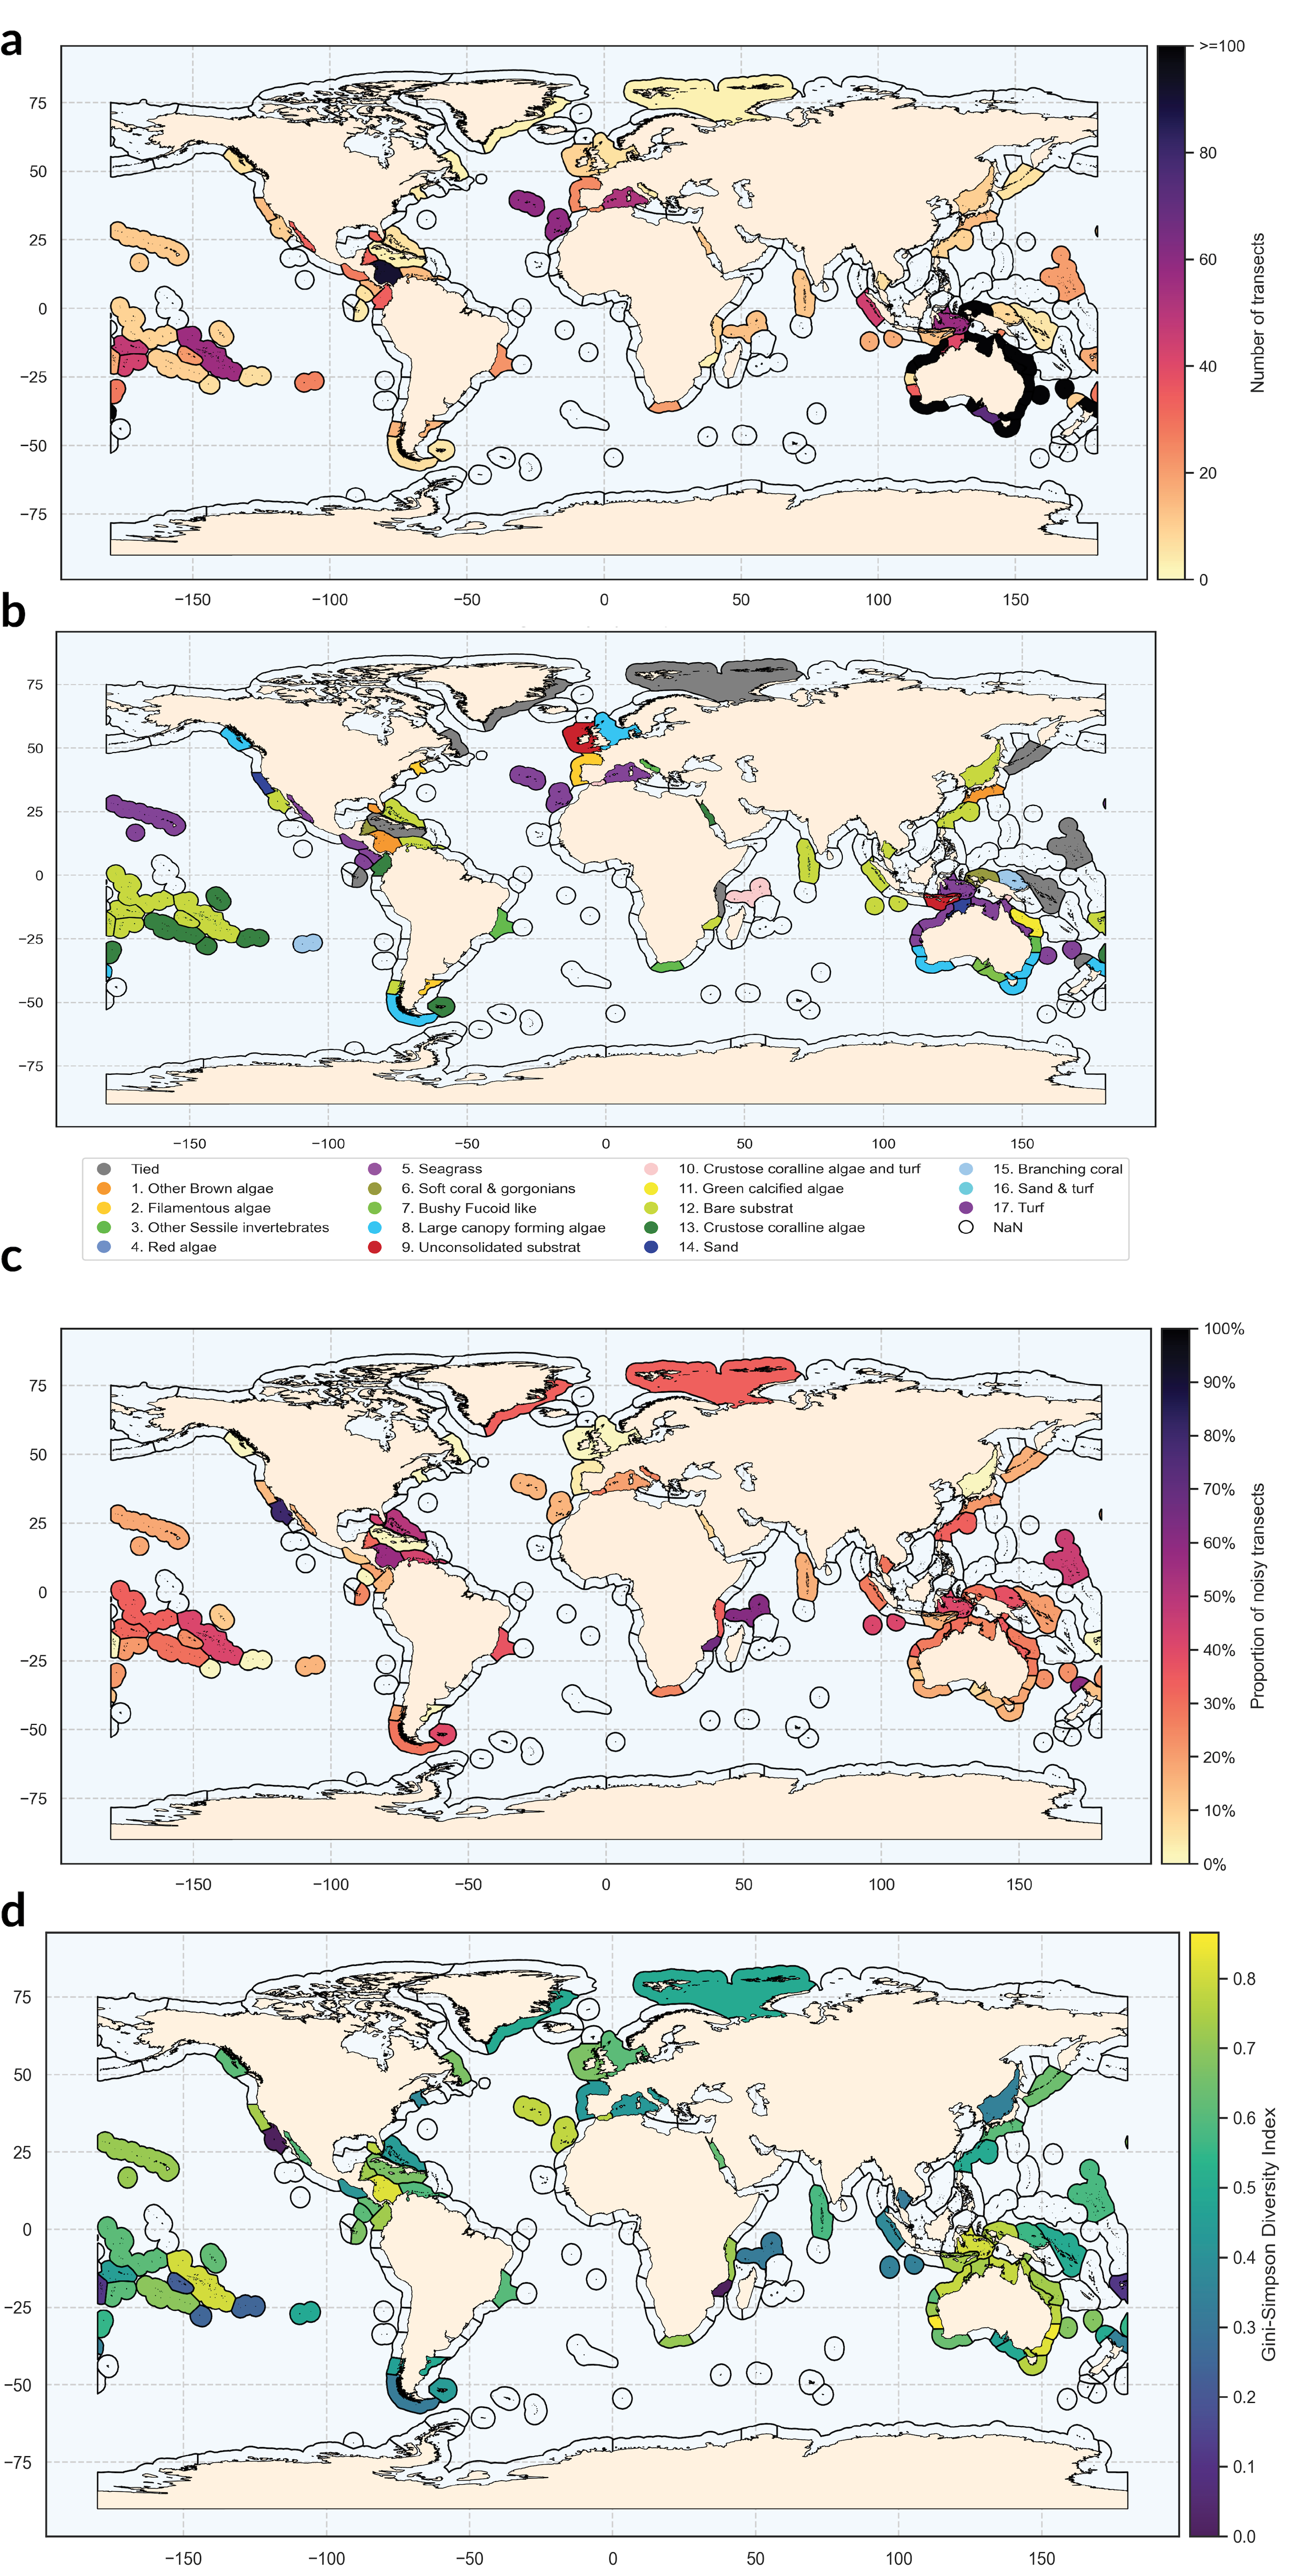
\includegraphics{03-Chapitre1/figures/fig4.png}
\caption[Change in explained variance related to environmental
predictors and random effects for three alternative model structures]{Change in explained variance related to environmental
predictors (left column) and random effects (right column) for three
alternative model structures (yellow for \emph{Phylogeny} (\emph{Ph}),
red for \emph{Traits and phylogeny} (\emph{TrPh}), and green for
\emph{Whole community} (\emph{WhC}) models) relative to the
\emph{Benchmark model} (\emph{Bench}; purple). Percentage changes were
computed relative to the \emph{Benchmark model} fitted with
presence/absence (top panels) or abundance (bottom panels) data.
Positive values indicate an increase in the proportion of variance
explained by the focal model compared to the \emph{Benchmark model}. See
Figure S23 and S24 for the raw percentages, expressed as percentages of
explained variance or total amount of variance
respectively.}\label{fig:chapt1fig4}
}
\end{figure}

\hypertarget{species-niche-estimated}{%
\subsection{Species niche estimated}\label{species-niche-estimated}}

For abundance models, the large majority (\textgreater60\%) of flat
response curves indicated a lack of meaningful species-environment
relationships (Fig.~\ref{fig:chapt1fig5}). This proportion reached 83\%
for the \emph{WhC} model. The prevalence of flat relationships did not
appear to be related to convergence issues (Fig. S15-16) or to be driven
by a specific covariate (Fig. S25). Convex or concave response curves
were rare in abundance models. Significant relationships primarily
included constant or accelerated declines, representing approximately
10\% and 15\% of response curves in the \emph{Bench}, \emph{TrPh}, and
\emph{Ph} models (Fig.~\ref{fig:chapt1fig5}). In the \emph{WhC} model,
these percentages decreased to 7\% and 6\%, respectively
(Fig.~\ref{fig:chapt1fig5}). Similar findings were observed for
presence/absence models (Fig. S26; Fig. S27).

\begin{figure}
\hypertarget{fig:chapt1fig5}{%
\centering
\includegraphics{03-Chapitre1/figures/fig5.png}
\caption[Number and proportion of response curves shapes.]{Number (y-axis) and proportion (computed across all
coefficients for each model, as indicated above individual bars) of
response curves (i.e.~one for each species-predictor combination
according to the typology (nine shapes highlighted by the black curve in
each panel) defined by \textcite{Rigal_2020}). Results are presented for
the different model structures}\label{fig:chapt1fig5}
}
\end{figure}

Both abundance and presence/absence \emph{TrPh} models (which include
species functional traits) reveal some meaningful trait-environment
relationships between the first fuzzy-PCA axis and the seven
environmental predictors. This suggests that the occurrence of certain
traits is likely favored (or hindered) under certain environmental
conditions (Fig. S28). For instance, mobile predatory species showed
larger declines in abundance as fetch increases than sessile
suspensivores (Fig. S28). Moreover, increase in organic matter
concentration and decrease in current velocities were associated with
higher abundances of suspensive feeders.

\hypertarget{exploring-the-residual-correlation}{%
\subsection{Exploring the residual
correlation}\label{exploring-the-residual-correlation}}

Residual species-species correlations were compared between the
\emph{Bench} model and the \emph{WhC} model, only for the 99 target
species, using both presence/absence (Fig S29) and abundance data
(Fig.~\ref{fig:chapt1fig6}). We only focus this comparison on the
\emph{WhC} model (rather than other models) because of its higher
predictive performance and higher proportion of explained variance by
random effects (Fig.~\ref{fig:chapt1fig4}). Residual correlations
estimated from both models were highly correlated, both for
presence/absence and abundance data (Fig.~\ref{fig:chapt1fig6} and Fig.
S29). However, agreement between models varied across different random
effects from a moderate correlation between residuals associated with
the Habitat random effects (\(\text{R}^2=0.57\)) or with the Site random
effects (\(\text{R}^2=0.64\)), to a high correlation between residuals
related to the Year random effects (\(\text{R}^2=0.95\)). The \(\delta\)
index main modal distribution, which is centered on zero, confirms an
overall agreement between residual correlations estimated from both
models in relation to the Year random effects with a marginal proportion
of sign changes (0.45\% of sign changes related to correlation greater
than 0.25; Fig.~\ref{fig:chapt1fig6} B) only related to low
species-species residual correlations (\textless0.25;
Fig.~\ref{fig:chapt1fig6} A and Fig. S29). In contrast, the \(\delta\)
index highlights inconsistencies in both magnitude and signs changes
between residuals associated with the Habitat and the Site (12.2\% and
9.11\% of sign changes related to correlation greater than 0.25) random
effects. Similar results were obtained for presence/absence models (Fig.
S29).

\begin{figure}
\hypertarget{fig:chapt1fig6}{%
\centering
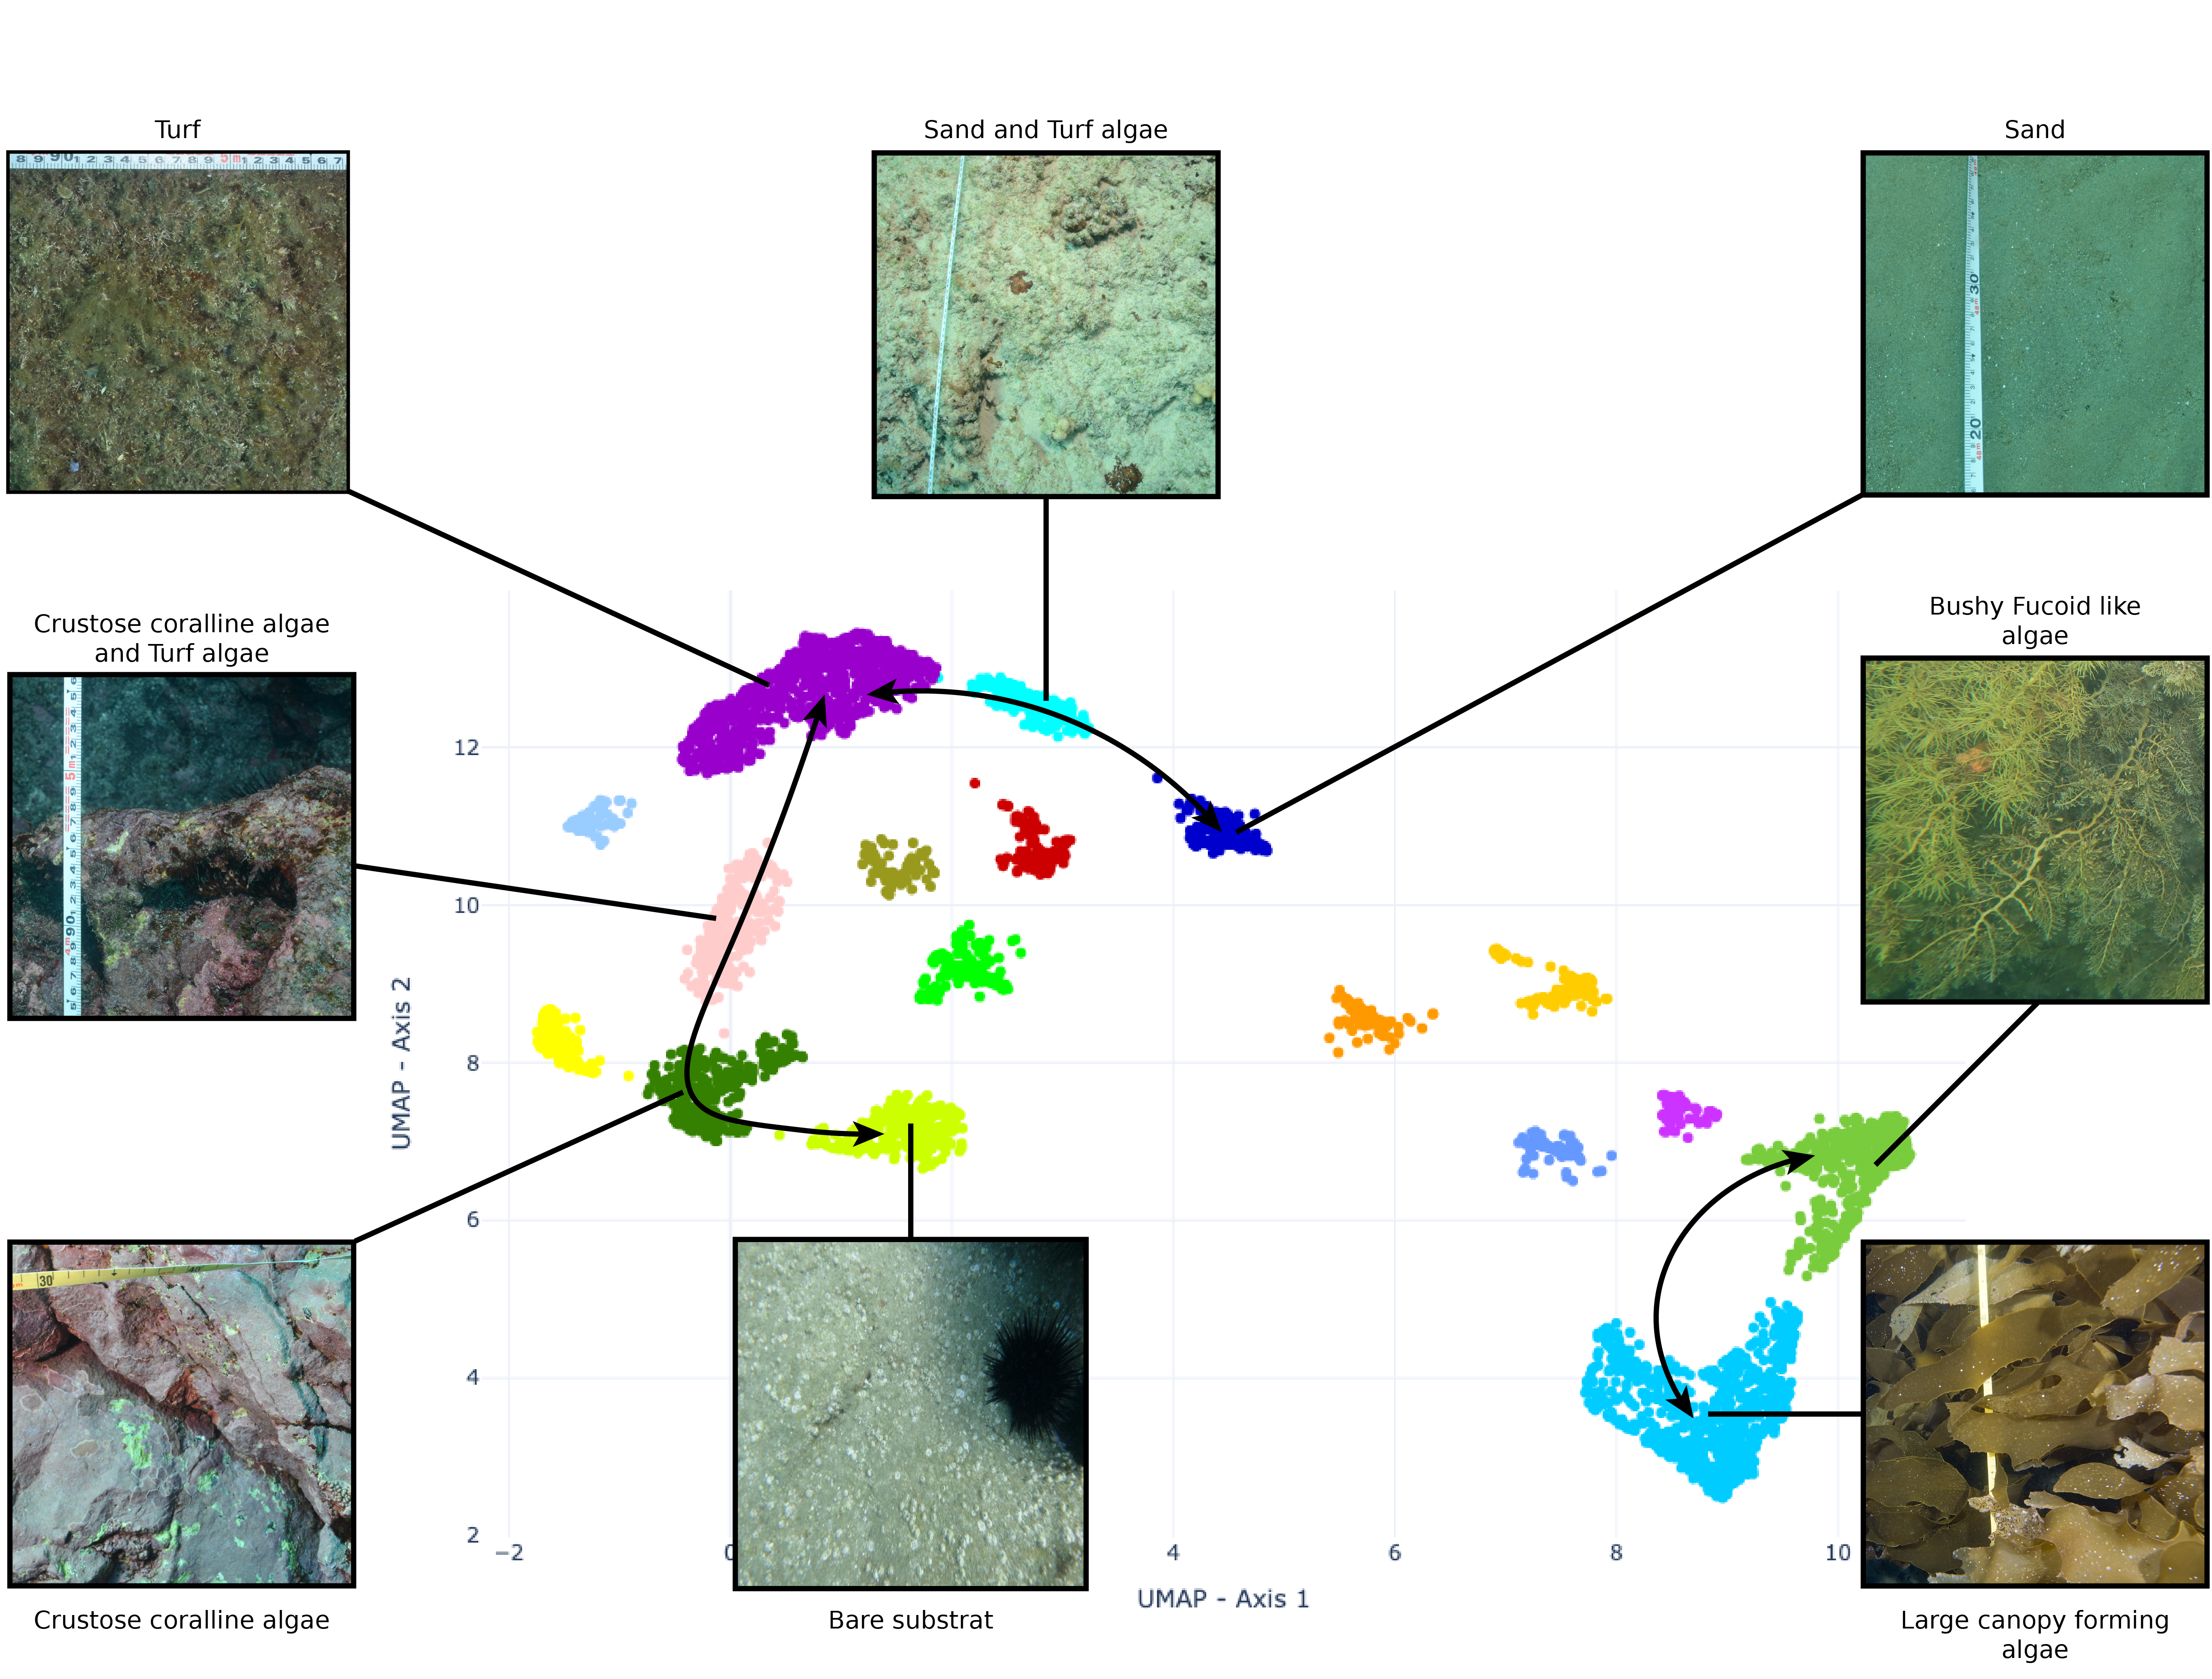
\includegraphics{03-Chapitre1/figures/fig6.png}
\caption[Comparison of residual species-species correlations
associated with the three random effects estimated by the \emph{Whole
Community Model}. (B) Distribution of the \(\delta\) index characterizing change in sign 
and magnitude between residual correlations estimated by
the \emph{WhC} model and the \emph{Bench} model]{(A) Comparison of residual species-species correlations
associated with the three random effects estimated by the \emph{Whole
Community Model} (\emph{WhC}; y-axis) and the \emph{Benchmark model}
(\emph{Bench}; x-axis) fitted on abundance data. The colour scale
highlights the density of points in each scatter plot. (B) Distribution
of the \(\delta\) index characterizing change in sign (negative values
indicate sign change) and magnitude (higher absolute values indicate
higher numerical difference) between residual correlations estimated by
the \emph{WhC} model and the \emph{Bench} model adjusted with abundance
data for the three random effects (Habitat, Site,
Year).}\label{fig:chapt1fig6}
}
\end{figure}

\clearpage

\hypertarget{discussion}{%
\section{Discussion}\label{discussion}}

Case studies in community ecology typically rely on partial and
heterogeneous observations \autocite{Pollock_2020} but also on
incomplete knowledge of target species ecological features (e.g.~traits,
phylogeny; \textcite{Tyler_2012}). This study investigated how
\emph{jSDM} performance varies depending on the type of information
included (i.e.~phylogeny, traits or data on non-target species) using a
multi-assessment framework (spanning interpretability, inference and
prediction, for both species- and community-level metrics, Table 1)
enabling a thorough evaluation of model performance.

We found that \emph{jSDMs}' performance, in particular predictive power
of abundance models at the species level, mostly increased when
including information related to the 179 non-target species sampled
alongside with the 99 polychaetes of interest. However, improvement in
species-level predictions does not directly translate into enhanced
performance at the community level. The \emph{WhC} model did not improve
estimates of beta diversity or total abundance relative to the other
models and largely overpredicted species richness, as previously
suggested \autocite{Zurell_2018}. Given \emph{HMSC} hierarchical
structure \autocite{Poggiato_2021}, inclusion of monitoring data related
to other species likely improves model performance for the target
assemblage by capturing relevant drivers that are not explicitly
considered. For instance, it can help describe target species' realized
niches by accounting for ecological processes related to environmental
conditions (including trait-mediated responses) or biotic interactions
that are not explicitly captured otherwise \autocite{Ovaskainen_2017a}.
In our case, main differences between residual correlations estimated by
the \emph{Benchmark model} and the \emph{Whole community} model relate
to spatial random effects (i.e.~site and habitat). In contrast, the
temporal random effect yielded similar residual co-occurrences in both
models. This suggests that including non-target species in our case,
mostly helped capture spatial variability in species associations across
sites and habitats.

Importantly, while we show that including non-target species can improve
predictive performance, in particular for rare species, benefits of
accounting for non-target species might vary depending on robustness of
non-target species monitoring data (e.g.~detection issues), their role
within the ecosystem (e.g.~engineer species are likely more influential
on local communities than rare transient species), or processes shaping
the target assemblage (if influence of abiotic factors dominates, then
adding other species will have marginal consequences on model
performance). While the list of additional species to consider can be
prioritized based on existing knowledge in well-studied ecosystems, such
information is often unavailable. Furthermore, a specific investigation,
that might rely on simulated datasets to overcome limitations related to
real world datasets \autocite{DiRenzo_2022}, would be required to
determine specific criteria, as well as optimal number of non-target
species to include. While species communities and assemblages are
largely defined arbitrarily \autocite{Stroud_2015}, a systematic
assessment of \emph{jSDM} performance as increasing the number and types
(for instance based on their functional or trophic roles) of non-target
species would be valuable to optimise model performance for the species
of management interests.

\emph{jSDMs} have already been used to model the distribution of a wide
variety of species ranging from micro-organisms \autocite{Minard_2019}
to megafauna \autocite{Brimacombe_2020} inhabiting many different
ecosystems. Here, while we studied assemblages associated with two
specific coastal habitats, i.e.~seagrass and sand, that have original
characteristics as they are located at the land-sea interface
\autocite{Boye_2019a}, our case study reflects typical aspects of
applied ecological research. These include issues related to data
limitation and availability but also typical features of ecological
communities (e.g.~prevalence of rare and transient species;
\textcite{Magurran_2003}) ; \textcite{SnellTaylor_2018}). Valuable
insights on trait-environment relationships are scarce in our study,
which reflects how contributions of functional ecology in \emph{jSDMs}
are likely limited by trait data quality and availability \autocites[
]{Tyler_2012}{deJuan_2022}. For instance, we found an interaction
between trophic modalities (i.e.~microphagous versus macrophagous diet)
and fetch (Fig. S15), indicating that organisms that filter on small
particles are less likely to occur in wave-exposed sites where high
levels of sediment resuspension can block their filtering systems
\autocite{Manning_2014}. Yet, the limited number of informative
trait-environment relationships or species-environment relationships
either suggest that neutral processes may shape polychaete assemblages
\autocite{Boye_2019a}; or rather highlight a mismatch between trait
data, environmental data, and the ecological processes at play
\autocite{deJuan_2022}. For instance, environmental variables only
capture mean climatological conditions, but fail to quantify variability
in the coastal environment, such as extreme events and seasonal or
annual variability. Likewise, the list of available fuzzy-coded traits
only partially captures species capacity to adapt to environmental
variability \autocite{deJuan_2022}. Thus, effectiveness of inclusion of
traits in \emph{jSDMs} is likely to be limited, or to rely on effort to
collect relevant trait information. In our case, while including traits
does not improve model predictive power, it somehow enhances our
understanding of species responses along environmental gradients. Hence,
if the goal is not prediction but inference \autocite{Tredennick_2021},
including traits and proxies of phylogeny can facilitate \emph{jSDM}
interpretation.

This paper lays out an original framework to systematically compare
multiple facets of alternative \emph{jSDM} formulations (i.e.~including
phylogeny, traits or additional species) on model interpretability,
explanatory and predictive power (Table 1). Using a set of complementary
metrics, we specifically assess performance of alternative model
formulations fitted to presence-absence or abundance data at the species
and community levels. Our framework goes beyond existing guidelines
proposed to assess the performance of \emph{jSDM} fitted on
presence-absence data \autocite{Wilkinson_2020} or that focus on the
predictive power of abundance-based models (e.g.
\textcite{Waldock_2022}). It specifically compares the performance (both
explanatory and predictive) and interpretability of alternative models'
formulations accounting for the multiple and high-dimensional components
that are typical of \emph{jSDMs}, namely: (1) species and community
level predictions including alpha and beta diversity metrics and ranking
of predictions according to species prevalence/abundance; (2)
species-environment relationships where we transposed the framework
initially developed for time series by \textcite{Rigal_2020} into an
effective tool to classify response curves according to 9 categories
across high numbers of species (e.g.~99 in our case study); (3)
trait-environment relationships; and (4) residual species-species
correlations associated with random effects thanks to a new index that
summarizes both changes in the sign and magnitude of the residual
correlations.

Overall, our results provide new insights into the most appropriate
strategies for \emph{jSDM} fitting, according to modelling objectives
\autocite{Tredennick_2021} and available data. While the four models
considered had similar explanatory power, adding extra information to
standard \emph{jSDMs} that only consider abiotic predictors can prove
useful in cases. For instance, adding monitoring data for other
non-target species can substantially increase model predictive power by
modifying inferred species-environment relationships and residual
correlation matrices. Similarly, adding traits or phylogeny can improve
model interpretability. Future studies will be key to consolidate our
findings on simulated case studies \autocites[
]{Zurell_2010}{DiRenzo_2022}, or across contrasted ecosystems, for
instance dominated either by environmental filtering, or by competitive
processes. Generalizing this approach across ecosystems will further
help prioritize data collection effort on the long term. For this
purpose, we recommend using a multi-model inference framework similar to
the one used in this study to systematically assess trade-offs
associated with alternative jSDMs formulations.

\clearpage

\printbibliography[heading=subbibintoc, title={Bibliographie}]
\end{refsection}
\printbibliography[heading=subbibintoc, title={Bibliographie}]
\clearemptydoublepage

\input{./03-Chapitre2/chapitre2}
\printbibliography[heading=subbibintoc, title={Bibliographie}]
\clearemptydoublepage

\begin{refsection}

\hypertarget{patterns-of-co-occurrence-and-spatial-richness-in-marine-habitats-insights-from-large-scale-modelling}{%
\chapter{Patterns of Co-occurrence and Spatial Richness in Marine
Habitats: Insights from Large-Scale
Modelling}\label{patterns-of-co-occurrence-and-spatial-richness-in-marine-habitats-insights-from-large-scale-modelling}}

\hypertarget{preambule-chapter3}{%
\section*{Préambule}\label{preambule-chapter3}}
\addcontentsline{toc}{section}{Préambule}

Grâce au Chapitre 2, nous avons identifié différents états d'habitats
biogéniques à l'échelle mondiale en appliquant une nouvelle méthode
d'agrégation que nous avons appliquée à des données d'un programme de
sciences participatives. Maintenant que les états d'habitats ont été
définis, ce chapitre vise à modéliser leur distribution à l'aide d'une
approche spatiale semblable à celle utilisée dans le cadre des
\emph{SDM}. Nous avons choisi de recentrer ces analyses du Chapitre 3
sur la région australo-pacifique, cœur géographique historique du
programme \emph{Reef Life Survey} \autocite{Edgar_2009}. L'objectif
premier est de comprendre les facteurs environnementaux et anthropiques
influençant leurs occurrences. En caractérisant les niches
environnementales, un second objectif est de déterminer les habitats
partageant des niches similaires donc susceptibles de coexister le long
des côtes australiennes. Dans ce contexte, ce chapitre vise à étudier la
distribution de 14 états d'habitats sur les côtes australiennes.

Nous avons utilisé un \emph{SDM} de type \emph{Random Forest} multivarié
pour caractériser les niches environnementales des états d'habitats en
considérant comme prédicteurs des données environnementales
(\emph{Bio-Oracle}; \textcite{Assis_2018}), et des données de pressions
anthropiques (\emph{Ocean Health Index} ; \textcite{Halpern_2019}). Nos
résultats indiquent que le modèle a un bon pouvoir explicatif, mais un
pouvoir prédictif faible, laissant penser que la transférabilité de
notre modèle dans le temps et l'espace est restreinte. Nos résultats
indiquent que les facteurs les plus importants régissant la distribution
de ces différents états d'habitats sont la température de surface de
l'eau, l'intensité de la pression de pêche et les anomalies dans la
fréquence des vagues de chaleur marine. Nous montrons également dans ce
chapitre que tous les états d'habitat identifiés ne pouvaient co-exister
dans le même transect ce qui suggère que certaines combinaisons d'états
d'habitats sont invraisemblables (ou jamais observées à ce jour). Ce
travail a permis également de mettre en avant que les zones de
transitions tempérées/tropicales sont susceptibles d' abriter un plus
grand nombre d'états d'habitats. Cela peut impliquer que ces zones sont
plus exposées aux changements de régime, puisque la disparition de
l'état dominant actuel pourrait laisser place au développement d'un état
d'habitat différent, notamment dans un contexte de tropicalisation des
zones tempérées chaudes des côtes est \autocites[
]{Verges_2014}{Verges_2019} et ouest \autocite{Wernberg_2016}
australiennes. Ces changements sont d'autant plus importants à
surveiller puisqu'ils pourraient avoir un impact important sur la
composition et les fonctions des communautés associées et par conséquent
modifier le fonctionnement même des écosystèmes.

Ce chapitre de thèse est l'oeuvre de la collaboration de Clément Violet, Aurélien Boyé, Mathieu Chevalier et de Martin Marzloff.

\clearpage

\hypertarget{abstract-chapt3}{%
\section{Abstract}\label{abstract-chapt3}}

Benthic reef habitats serve as foundational structures in coastal
ecosystems, facilitating essential ecological processes and
significantly amplifying biodiversity. However they are increasingly
subject to regime shifts that can be detrimental for marine ecosystem
functioning and biodiversity. In this study we aim to investigate the
distribution and ecological drivers of reef benthic habitat states
across Australia, in order to understand and anticipate their
potential/risk of ecological regime shifts in the face of changing
environments and anthropogenic impacts. Using random forest models
applied to occurrences of reef habitat states stemming from a previous
analyses of the \emph{Reef Life Survey} transect data, we quantified the
relative contribution of anthropogenic and environmental drivers in
explaining their spatial distribution. Specifically, we focused on 14
reef states including turf, kelp or coral reefs. Models showed a good
explanatory power with AUC (\(\text{mean} = 0.87\);
\(\text{sd} = 0.07\)). For most habitats, we found that SST, Fishing
intensity and Marine Heatwaves were the most important driver of their
distribution while anthropogenic factors only had a marginal influence.
However, models presented a poor predictive power suggesting limited
transferability in time or space. On the calibration areas, we found
that several habitats (up to eight) can occur under similar
environmental conditions, suggesting that the likelihood of state
changes (including regime shifts) is spatially variable. Overall, this
approach makes it possible to highlight areas and environmental
conditions where the occurrence of alternative stable states is more
likely.

\clearpage

\hypertarget{intro-chapt3}{%
\section{Introduction}\label{intro-chapt3}}

Regime shifts are persistent changes in the structure and/or the
function of ecosystems occurring more or less suddenly \autocites[
]{Scheffer_2001}{Scheffer_2003}. Ecological regime shifts have been
identified in many different ecosystems: forest to savannahs
\autocite{Staver_2011}, tundra to boreal forests
\autocite{Scheffer_2012}, coral reefs to macroalgae dominated reefs
\autocite{McManus_2004}, or fisheries collapse \autocite{Gardmark_2015}.
Areas affected by regime shifts tend usually display profound and
lasting changes in the ecosystem services they provide to human
populations \autocite{Rocha_2015a}, with economic impacts through the
disappearance of certain activities \autocite{Crepin_2012}, and societal
and cultural impacts through the loss of cultural and traditional
knowledge \autocite{Mustonen_2021}. Thus, one of the common features of
all these regime shifts is that they drive the ecosystem under
consideration towards a new state, considered from a human perspective
to be less desirable \autocite{Scheffer_2009bk}.

Multiple factors can trigger a change in ecological regime towards a new
ecosystem states \autocite{Rocha_2015b}. These factors include climatic
variations caused by global climate change \autocite{Rocha_2015b},
increase in the number of extreme climatic events
\autocite{Wernberg_2016}, introduction of invasive species
\autocite{Kotta_2018}, increase in anthropogenic pressure
\autocite{Halpern_2019}, and loss of biogenic habitats
\autocite{Airoldi_2008}.

Biogenic habitats, formed by engineers' species, play a crucial role in
the functioning of marine coastal ecosystems and in supporting
components of biodiversity \autocites[ ]{Vozzo_2023}{Albertson_2022}.
For instance, mangroves serve as a nursery for coral-reef fish
\autocite{Nagelkerken_2002}, coral act as a refuge from predators for
many fish and invertebrates species \autocite{Almany_2004}, marine
seagrasses enhance water quality by for instance increasing water pH
\autocite{Ricart_2021}, and their presence increases infauna diversity
\autocites[ ]{Gonzalez-Ortiz_2016}{Boye_2017}. Because biogenic habitats
are also vulnerable to human pressures and natural disturbances
\autocites[ ]{Airoldi_2007}[ ]{Butt_2022}{Wernberg_2023}, they play a
central role in mediating the effects of current environmental changes
on marine coastal ecosystems and biodiversity \autocites[
]{Sunday_2017}{Bulleri_2018}.

Over the last few decades, regime shifts involving persistent changes in
biogenic benthic habitats have been observed worldwide across temperate
and tropical regions. Examples include shifts from macroalgal forests to
either sea urchin barrens \autocite{Ling_2015} or turf
\autocite{Filbee-Dexter_2018}, from crustose coralline algae to turf
\autocite{Cornwall_2023}, and also from coral-dominated reefs to
macroalgae \autocite{McManus_2004}, or from seagrass to bare sediments
\autocite{Maxwell_2017}. These regime shifts share in common that as the
biogenic habitats degrade or change, novel ecological dynamics take root
to push and maintain the ecosystems into new states
\autocite{Nystrom_2012}. As these new states are often undesirable from
a management perspective while also displaying hysteresis making it
difficult to return to the initial state \autocite{Nystrom_2012},
substantial efforts have been devoted to identifying, predicting and
preventing regime shifts before they occur \autocite{Biggs_2009}.
Detection of early warning signals of regime shifts has been intensively
investigated by analysing temporal ecosystem dynamics when long-term
time series are available \autocite{Scheffer_2009}, or spatial patterns
emerging from ecological dynamics \autocites[ ]{Kefi_2014}[
]{Nijp_2019}{Ward_2018}. Although promising theoretically based on
numerical or mesocosm experiments, these data-greedy methods remain of
limited practical interest in real world ecosystems across large spatial
scales , as (i) they are often computed retrospectively after the shift
has occurred (e.g. \textcite{Litzow_2014}) and (ii) to date, no single
metrics amongst the alternative candidates (e.g.~increasing variance,
skewness, etc\ldots) has proven reliable across all case studies
\autocite{Hastings_2010}. An alternative that has gained increasing
interests is to identify the environmental thresholds beyond which
ecosystems shift to new states \autocite{Kelly_2015}. However, this
approach has also proved challenging \autocites[
]{Turner_2020}{Hillebrand_2020}. Process-based simulation models can for
instance contribute to estimating ecological thresholds and informing
effective management strategies \autocites[
]{Marzloff_2013}{Marzloff_2016} but they remain restricted to
theoretical cases or data-rich ecosystems. Overall, different strategies
may be necessary to anticipate regime shifts across ecosystems,
depending on data availability and ecosystem properties (e.g.~non-linear
responses, lags in response to effects of stressors ;
\textcite{Litzow_2016} ; \textcite{Turner_2020}).

In the case of coral reefs, defining and modelling the occurrence of
alternative reef states have improved our understanding and ability to
predict the impact of anthropogenic pressures on reef states \autocites[
]{Jouffray_2015}[ ]{Jouffray_2019}{Donovan_2018}. After identifying
potential reef states (e.g. \textcite{Donovan_2018} ; Chapitre 2),
modelling their spatial distribution can indeed help assess the relative
importance of different environmental drivers (including climate-driven
or local anthropogenic pressures), evaluate the extent to which drivers
have synergistic or antagonistic effects on ecosystem states, and also
characterise potential non-linear ecosystem responses across
environmental gradients \autocites[ ]{Jouffray_2015}{Jouffray_2019}. All
these elements are key to guide anticipatory strategies and define
management actions \autocites[ ]{Litzow_2016b}{Turner_2020}. An
unexplored avenue concerns the potential for distribution models to
identify areas where multiple ecosystem states are possible and hence,
where supposedly changes in ecosystem states are more likely. To date
however, such modelling strategy has only been led on coral reefs at a
local scale \autocite{Jouffray_2019} so its transposability to other
ecosystems across larger areas remains untested.

In this context, Chapter 2 defined habitat states using the \emph{Reef
Life Survey} (\emph{RLS}) database, which provides a solid basis for a
modelling exercise on a regional scale. Building on the dataset of reef
states occurrences around Australia consolidated in Chapter 2, this
study aims to explain and predict their distribution using SDM
approaches, with the specific goals of (1) assessing the influence of
biophysical factors and anthropogenic pressures on the occurrence of the
different reef habitat states, (2) determining the transferability of
these SDMs in order to quantify the predictability of reef habitat
states at large scales, (3) identify reef states that share similar
environmental niches and can potentially coexist, and (4) identify
areasthat may host several states, as these areas are the most likely to
undergo state changes.

\clearpage

\hypertarget{mat-met-chapt3}{%
\section{Materials \& Methods}\label{mat-met-chapt3}}

\hypertarget{datasets}{%
\subsection{Datasets}\label{datasets}}

\hypertarget{biotic-dataset}{%
\subsubsection{Biotic dataset}\label{biotic-dataset}}

In this study, we used the dataset produced in Chapter 2 from the
\emph{RLS} citizen science program where 50-m diver transects were
classified into different habitat states based on percentage cover
estimates of major benthic habitat groups. As a reminder of Chapter 2,
we used a clustering pipeline composed of two distinct algorithm
\emph{UMAP} \autocite{McInnes_2020} for dimension reduction and
\emph{HDBSCAN} \autocites[ ]{Moulavi_2014}{McInnes2017} to classify the
\emph{RLS} benthic habitat relative cover (estimated through underwater
dives; for further details see \textcite{Edgar_2014}) for 6,554
transects into 17 distinct states. These 17 reef states include iconic
biogenic habitats such as kelp forests, encrusting red algae, corals,
and seagrass beds, as well as alternative degradation states of these
habitats (i.e.~branching coral vs.~turf algae). Out of the 6,554
transects classified, 5,122 were sampled in Australian waters, which are
the focus of this study. Not that this classification methodology
excludes certain observations considered as noisy. Thus, from this
dataset, we removed all transects classified as ``noisy'' (935
transects) while also removing transects for which at least one
covariate had missing value due to the immediate proximity of the
coastline (871 transects). Thus, the following analyses are based on
3,316 transects. As our goal in this study is to understand the
distribution of biogenic habitats, we merged three out of the 17 initial
habitat states (i.e.~``Unconsolidated substrat'', ``Bare substrat'' and
``Sand'') into a single group that corresponds to non-living substrate
(``Substrate'' hereafter). In addition, since turf algae can trap
sediments and produce chemical substances preventing the recruitment of
canopy-forming species \autocite{Burek_2018}, we decided to merge the
initial group ``Sand and Turf algae'' with the group ``Turf algae''.
Overall, 14 reef states are modelled in this study (See appendix A,
Table S1 for their description and Fig. S1 for their distribution across
the dataset).

\hypertarget{predictors-dataset}{%
\subsubsection{Predictors dataset}\label{predictors-dataset}}

The predictors used for model fitting were extracted from two sources:
\emph{Bio-Oracle} \autocite{Assis_2018} for biophysical predictors and
\emph{Ocean Health Index} \autocite{Halpern_2019} for anthropogenic
pressures. \emph{Bio-Oracle} provides aggregated data for the period
2000-2014 at a resolution of 0.083° (9.28 km at the equator). From this
database, we extracted the mean values of four biophysical predictors
known to be important for coastal ecosystems
(Table~\ref{tbl:chap3tbl1}).

The Ocean Health Index database provides yearly estimates for 14
predictors for the period 2003-2013 at a resolution of 0.0083° (928 m at
the equator). We extracted yearly data for the eight predictors known to
impact coastal ecosystems and computed the mean for all predictors. We
also computed the standard deviation for the predictors linked to
fishing activity (i.e.~Artisanal fishing, Fishing High and Low Bycatch,
Fishing Non-Destructive High and low Bycatch) . We then performed a
principal component analysis on all predictors related to fisheries so
as to synthesise the core information related to fishing impacts. The
first two axes explained 44.3\% and 21.3\% of the variability,
respectively. The first axis mostly describes variation in the intensity
of destructive fishing activity for marine benthic habitats, whereas the
second axis is related to non-destructive fishing activity (See Fig. S2
appendix A). In addition, we ensured that the selected predictors were
not too highly correlated with each other (all absolute values of
Pearson's correlations \textless{} 0.7 ; Fig. S3 in appendix A).

\clearpage

\hypertarget{tbl:chap3tbl1}{}
\begin{longtable}[]{@{}
  >{\centering\arraybackslash}p{(\columnwidth - 4\tabcolsep) * \real{0.2170}}
  >{\raggedright\arraybackslash}p{(\columnwidth - 4\tabcolsep) * \real{0.3774}}
  >{\centering\arraybackslash}p{(\columnwidth - 4\tabcolsep) * \real{0.3962}}@{}}
\caption[Environmental variables extracted from
\emph{Bio-Oracle} and anthropogenic variables extracted from \emph{Ocean
Health Index}.]{\label{tbl:chap3tbl1}Environmental variables extracted from
\emph{Bio-Oracle} and anthropogenic variables extracted from \emph{Ocean
Health Index}. See \textcite{Assis_2018} for a detailed description of
the \emph{Bio-Oracle} variables and their acquisition method and Table
S1 to S3 in \textcite{Halpern_2019} for detailed description and
acquisition method of anthropogenic variables}\tabularnewline
\toprule\noalign{}
\begin{minipage}[b]{\linewidth}\centering
\textbf{Data source}
\end{minipage} & \begin{minipage}[b]{\linewidth}\raggedright
\textbf{Variable}
\end{minipage} & \begin{minipage}[b]{\linewidth}\centering
\textbf{Metric}
\end{minipage} \\
\midrule\noalign{}
\endfirsthead
\toprule\noalign{}
\begin{minipage}[b]{\linewidth}\centering
\textbf{Data source}
\end{minipage} & \begin{minipage}[b]{\linewidth}\raggedright
\textbf{Variable}
\end{minipage} & \begin{minipage}[b]{\linewidth}\centering
\textbf{Metric}
\end{minipage} \\
\midrule\noalign{}
\endhead
\bottomrule\noalign{}
\endlastfoot
\multirow{4}{*}{\emph{Bio-oracle}} & Current velocity &
\multirow{4}{*}{Mean} \\
& Diffuse attenuation \\
& Primary productivity \\
& Sea Surface Temperature \\
\hline
\multirow{8}{*}{\emph{Ocean Health Index}} & Artisanal Fishing &
\multirow{5}{*}{\small PCA axis on Mean and Standard deviation} \\
& Fishing High Bycatch \\
& Fishing Low Bycatch \\
& Fishing Non Destructive High Bycatch \\
& Fishing Non Destructive Low Bycatch \\
& Direct Human Disturbance\footnote{Coastal density population within a
  10 km radius of the coastline. See Table S1 and S2 in
  \textcite{Halpern_2019} supplementary information for more details.} &
\multirow{3}{*}{Mean} \\
& Nutrient Pollution \\
& Marine Heatwaves Anomaly\footnote{Marine Heatwaves Anomaly is
  calculated by subtracting the count of extreme sea surface temperature
  weeks during a five-year period from the count of extreme sea surface
  temperature weeks during a baseline five-year period (1985-1989). See
  Table S1 and S2 in \textcite{Halpern_2019} supplementary information
  for more details.} \\
\end{longtable}

Since the \emph{Bio-Oracle} and \emph{Ocean Health Index} datasets have
different resolutions and projections, all predictors were reprojected
to a common projection (EPSG:4326) and a common resolution of 0.0083°,
which is the highest resolution offered by \emph{Ocean Health Index}.
Hence, bio-oracle predictors were downscaled to match the \emph{Ocean
Health Indices} resolution.

\hypertarget{statistical-analyses}{%
\subsection{Statistical analyses}\label{statistical-analyses}}

\hypertarget{model-fitting-and-evaluation}{%
\subsubsection{Model fitting and
evaluation}\label{model-fitting-and-evaluation}}

We modelled habitat states using a multivariate Random Forest model
\autocite{Breiman_2001} fitted using the Python library Scikit-Learn
\autocite{scikit-learn}. The Random Forest model was trained on 163,800
combinations of hyperparameters ``\emph{max\_depth}'',
``\emph{max\_features}'', and ``\emph{n\_estimators}'' (see Table S2 in
appendix B). For each combination of hyperparameters, we binarised the
probabilities obtained from the Random Forest model according to reef
state-specific thresholds that maximized the True Skill Statistic
(MaxTSS ; \textcite{Allouche_2006}), and only retained combination of
hyperparameters having the highest MaxTSS on the explanatory folds (see
below for the train/test split of the dataset).

To address the proximity of some transects and the resulting spatial
autocorrelation, we used a 3-fold cross-validation procedure with
spatial blocks for model training. Using the \emph{blockCV} R package
\autocite{Valavi_2019}, the autocorrelation range of the presences and
absences between the different habitats states was estimated as 524
km\(^2\), which was then used to split our study area into 37 blocks of
that size (equal area across blocks) to ensure that the spatial
correlation between any two blocks was negligible. Finally, each block
and all the transects it contains were randomly assigned into three
folds. This whole procedure ensured that spatially close transects were
not used to both train and validate the model (See Fig S5. in appendix
A). Using this method, we allocated the 3,316 transects into three folds
that were used for training (and assessing explanatory power) as well as
for estimating predictive power (training with two folds to predict the
remaining one, in a classical cross-validation scheme). The distribution
of different habitat states within the different training and test folds
is presented in Fig S6 in appendix A.

The performance of explanatory power and predictive power were evaluated
using a set of complementary metrics including the maximum of the True
Skill Statistic (Max TSS) \autocite{Allouche_2006}, the F1-score, the
Area Under the Precision-Recall Curve (AUPRC) \autocite{Flach_2015} and
the AUC \autocite{Fawcett_2006}. Because model predictive power was
poor, tThe best hyperparameter combination based on explanatory power
was then used to fit the model on the whole dataset.

\hypertarget{model-predictions}{%
\subsubsection{Model predictions}\label{model-predictions}}

The most important variables in explaining the distribution of each reef
habitat state were identified using the \emph{SHAP} (\emph{SHapley
Additive exPlanations}) framework \autocite{Lundberg_2017}. is a
framework rooted in cooperative game theory \autocite{Shapley_1953} that
quantifies the contribution of each predictor to model predictions
\autocite{Lundberg_2017}. \emph{SHAP} values were then averaged across
states to identify the three most important variables across all states.
Then, for each habitat state, we modelled their dependence against these
three most influential variables using Partial Dependence Plots
(i.e.~marginal response curves; \textcite{Molnar_2022}) across the
observed range of our predictors.

Then, we investigated whether certain environmental conditions could be
suitable for multiple habitats. To this end, we used the threshold that
maximised the TSS for each habitat state during the hypertunning of the
parameters of the Random Forest model (Fig. S7), to binarise occurrence
probabilities into presences and absences. We then stacked these binary
predictions across habitats to compute the number of states predicted as
present in each pixel/set of environmental conditions. As performed for
individual reef states, we explored the response of this number of
predicted states against the three most influential variables,
identified above, using Partial Dependence Plots.

From the stacked predictions, we also identified the habitat states that
can co-occur in the same transect. We calculated the relative frequency
with which each habitat state was associated with zero, one, two or more
of the other habitat states. In order to study the spatial distribution
of the number of predicted habitat states, we further calculated the
minimal, median and maximum number of habitat states per spatial block.
That scale was chosen since spatial blocks were built to be uncorrelated
(and therefore independent) spatial units. Using a linear regression, we
then investigated whether these spatial summary statistics varied
depending on the coordinates of the spatial blocks (using the centroid
of the block), and the number of transects within each spatial block.
Quadratic effects were included for the latitude and longitude of the
spatial blocks in order to account for potential non-linear effects.

\clearpage

\hypertarget{results-chapt3}{%
\section{Results}\label{results-chapt3}}

\hypertarget{model-performance-predictors-importance}{%
\subsection{Model Performance \& Predictors
importance}\label{model-performance-predictors-importance}}

The models with the selected hyperparameters showed good explanatory
power (measured on the fold on which the model was trained) with an
average Max TSS across all habitat states of 0.78 ± 0.03 (mean ±
standard deviation; Fig. S6 in appendix B). AUC values ranged from 0.89
to 0.99 (Fig. S8-21 in appendix B), while AUPRC values ranged from 0.48
to 0.71 (Fig. S22-35). The best explanatory power according to maxTSS
was obtained for ``Soft coral and gorgonians'' (\(\text{TSS}=0.94\)),
while the worst was obtained for ``Turf'' (\(\text{TSS}=0.49\)). The
predictive power (calculated on the fold not used for model training)
was significantly worse, with a mean Max TSS of 0.13 ± 0.04 (mean ±
standard deviation).

Our results show that habitat states usually respond to a set of weak
predictors (i.e.~most predictors contributed similarly to the
explanatory power, although with some slight differences;
Fig.~\ref{fig:chap3fig1}). The three most important variables were Sea
Surface Temperature, Fishing PC1 and Marine Heatwave anomalies (see Fig.
S36-50 in appendix C). Although these three variables were the most
important considering all habitats, the occurrence of certain habitats
was best predicted by other covariates. For example, Primary
Productivity appeared as a relevant predictor of Crustose coralline
algae distribution, whereas Current Velocity was important for both
Filamentous algae (Fig. S42 in appendix C), and Seagrass (Fig. S47. in
appendix C). Overall, Direct Human Disturbance had a low explanatory
power for all habitat states.

\newpage

\begin{figure}
\hypertarget{fig:chap3fig1}{%
\centering
\includegraphics{03-Chapitre3/figures/04-states_hab_shap_matrix_normalized.png}
\caption[Heatmap of the relative contribution of variables to the Random
Forest explanatory power.]{Heatmap of the relative contribution of variables to the Random
Forest explanatory power. The variables are colour coded according to
the type of predictor (blue : abiotic conditions, green : fishing
pressure, orange : other anthropogenic pressures). The relative
contribution of each variable for a given state is expressed relative to
the sum of all variable's contributions for that
state.}\label{fig:chap3fig1}
}
\end{figure}

\hypertarget{habitat-states-patterns}{%
\subsection{Habitat states patterns}\label{habitat-states-patterns}}

Overall, stacking predictions showed that most conditions are suitable
to multiple habitat states, with a richness (i.e.~number of predicted
reef states for a given set of environmental conditions) of 3.43 ± 1.50
(mean ± standard deviation) ranging from one to eight potential habitat
states occurring per transect. The richness varied differently along
environmental gradients (Fig.~\ref{fig:chap3fig2} a): for instance,
large variations around an average richness value of 4 were observed for
Sea Surface Temperature whereas a global (non-linear) decrease was
observed when fishing pressure or Marine heat-wave anomalies increased.

Changes in habitat state richness along environmental gradients depends
on the response of the 14 reef habitat states along these gradients
(Fig.~\ref{fig:chap3fig2} b). Indeed, the relative stability of habitat
state richness along the mean temperature gradient does not reflect a
stability in the response of the different states but rather that some
states are replacing others at certain temperature values. For instance,
when Sea Surface Temperature exceeds 20°C, the model predicts a strong
decrease in the probability of occurrence of Canopy Forming algae and
Bushy Fucoid states but an increase in the probability of states
dominated by Crustose coralline algae with and without Turf and by Green
calcified algae. A bove that same 20°C threshold, the probability of
occurrence of the Turf state is maximal. With regards to fishing
pressure, the probability of occurrence of Large canopy forming algae
increases with fishing pressure. For Marine Heatwaves, while the
probability of occurrence Green calcified algae decreases as the
frequency of Marine Heatwaves increases, the opposite is observed for
Bushy Fucoid like states.

\begin{figure}
\hypertarget{fig:chap3fig2}{%
\centering
\includegraphics{03-Chapitre3/figures/08-pdp_shap_env_richness.png}
\caption[Partial Dependence Plots of the a. Habitat states richness b.
probability of each of the 14 habitat states against the three most
important variables identified.]{Partial Dependence Plots of the a. Habitat states richness b.
probability of each of the 14 habitat states against the three most
important variables identified previously for these habitat states,
namely: Sea Surface Temperature, Fishing PC1 (Fishing pressure increases
as Fishing PC1 increases) and Marine Heatwaves Anomaly. For all plots,
the X-axis is expressed in the original unit of the variables. For
graphical representation, we only plot here the {[}0\%; 90\%{]} values
of Fishing PC1, due to few positive extreme
values.}\label{fig:chap3fig2}
}
\end{figure}

Among the 3,316 transects analysed, 222 (\textasciitilde6.5\%) are
predicted to be only suitable to a single habitat state while 71\%
exhibit favourable conditions to accommodate two to four different
habitat states (Fig.~\ref{fig:chap3fig3} a). Out of the 16,384 possible
combinations of occurrence and co-occurrence of the 14 habitat states,
we predict only 302 (\textasciitilde2\%) combinations of co-occurring
habitat states. Among these combinations, 12 comprised one habitat state
(note that Brown algae as well as Soft coral and gorgonians were never
predicted to occur alone), while a maximum of 112 combinations were
observed in transects predicted to be suitable for three different
habitat states.

Interestingly, some reef habitat states (e.g.~Turf or Large canopy
forming algae) are more likely to occur in conditions suitable for only
a few habitat states (one or two habitat states) while others
(e.g.~Filamentous algae, Red algae, Brown algae and Other Sessile
invertebrates) are more likely to occur in conditions supposedly
favourable to a large number of habitat states (Fig.~\ref{fig:chap3fig3}
b).

Futher, our results indicate a preferential association between certain
habitat states (Fig.~\ref{fig:chap3fig3} c). For instance, some iconic
reef habitat states such as Branching coral are mainly predicted in
areas that are also favourable to Turf (19\% of the time) and Large
Canopy Forming algae (14\%). Other reef states such as Bushy Fucoidlike
are mainly associated with Large canopy forming algae (15\%), Turf
(12\%), Substrate (11\%), and Filamentous algae (11\%).

\begin{figure}
\hypertarget{fig:chap3fig3}{%
\centering
\includegraphics{03-Chapitre3/figures/05-multipanel_fig_ab.png}
\caption{a. Distribution of the number of possible habitat states per
transects, the numbers above the bar represent the number of transects
predicted to have this number of habitat states. b. Relative frequency
of habitat states as a function of predicted number habitat states in
one transect. c.~Heatmap of the frequency of co-occurrence of each
habitat state. Each line of the heatmap has been standardised by the
total number of co-occurrences with the focal habitat
state.}\label{fig:chap3fig3}
}
\end{figure}
\begin{figure}
\ContinuedFloat
\includegraphics{03-Chapitre3/figures/05-multipanel_fig_c.png}
\caption[]{a. Distribution of the number of possible habitat states per
  transects, the numbers above the bar represent the number of transects
  predicted to have this number of habitat states. b. Relative frequency
  of habitat states as a function of predicted number habitat states in
  one transect. c.~Heatmap of the frequency of co-occurrence of each
  habitat state. Each line of the heatmap has been standardised by the
  total number of co-occurrences with the focal habitat
  state.}
\end{figure}

\hypertarget{spatial-distribution}{%
\subsection{Spatial distribution}\label{spatial-distribution}}

At the Australian geographical scale, different spatial patterns of
richness (i.e.~number of predicted reef states) were observed depending
on the region (Fig.~\ref{fig:chap3fig4}). Most spatial blocks around
Australia have transects where only one unique habitat state can occur
(Fig.~\ref{fig:chap3fig4} a). The majority of spatial blocks have a
median richness of 3 (Fig.~\ref{fig:chap3fig4} b). One has a richness of
6, but the number of transects in this spatial block is relatively low,
with only seven transects sampled. On the east coast of Australia, in
the Tweed-Moreton and Manning-Hawkesbury ecoregions, two ecoregions at
the transition between temperate and tropical zones, the max richness
was 8 whereas the median value of the adjacent temperate or tropical
zones was lower. Over 73\% of spatial blocks can accommodate up to seven
or eight different reef habitat states (Fig.~\ref{fig:chap3fig4} c).
Only the maximum of predicted reef states showed a significant
relationship, albeit weak (linear coefficient of 0.007), with the number
of transects carried out (\(p<0.01\)).

\begin{figure}
\hypertarget{fig:chap3fig4}{%
\centering
\includegraphics{03-Chapitre3/figures/09-Spatial-block-diversity.png}
\caption{a. Minimal, b. median and c.~maximal richness (i.e.~number of
predicted reef states) per spatial block}\label{fig:chap3fig4}
}
\end{figure}

\clearpage

\hypertarget{discussion-chapt3}{%
\section{Discussion}\label{discussion-chapt3}}

In this study, we built upon Chapter 2 to explain and predict the
spatial distribution of multiple reef benthic habitats. Overall, the
random forest multivariate modelling approach we have used showed
substantial explanatory power but a low predictive power, suggesting
poor transferability. Despite evidence for a good explanatory power, all
predictors presented a similar contribution to the variance explained
precluding us to clearly identify the drivers of the spatial
distribution of most habitats. Partial dependence plots highlighted some
meaningful relationships and showed a differential response of habitats
along environmental gradients that may ultimately trigger the emergence
of alternative stable states. Importantly, some environmental conditions
appeared to be suitable for several habitats suggesting that the current
existence of an habitat in a given area may be due to historical
contingencies and/or biotic settings.

\hypertarget{explanatory-and-predictive-power-of-the-model}{%
\subsection{Explanatory and predictive power of the
model}\label{explanatory-and-predictive-power-of-the-model}}

Our model demonstrates some explanatory power, especially when it comes
to elucidating the distribution of the rarest habitat states in the
dataset such as Branching coral or Soft coral and gorgonians (See Fig.
S1 in appendix A and Fig. S6 in appendix B). This outcome suggests that
the model is able to decipher the reason why habitat states are absent
and gives us insight about the complex relationships between
environmental factors and habitat states. This strongly contrasts with
the model's predictive power, which is quite low overall. Several
factors may contribute to the low transferability of the models. First,
the reef habitat states defined in Chapter 2 are derived from cover data
of about 50 substratum types defined accordingly to the CATAMI benthic
imagery classification scheme (\textcite{Althaus_2015} ; for further
details, see \textcite{Edgar_2020}), merged into 24 functional group.
Hence, the initial reef state categorisation is based on cover data of
morpho-types that does not take into account the identity of the
underlying species. As a result, some reef states may have large
environmental niches in our model while they are in fact driven by
species with much narrower niches and located in different areas. For
example, the diversity of Crustose coralline algae is estimated at
several hundred different species \autocite{Dean_2015,Twist_2019}, which
can be found in both temperate and tropical zones
\autocite{Sissini_2022}. The same goes for Turf, which is a rather
loosely defined functional group \autocite{Connell_2014}. Turf can
include nearly a hundred different species, sometimes with a lack of
consistency in its definition across space \autocite{Connell_2014}.
Hence, while Turf can be found in both tropical and temperate zones, the
underlying species and their ecology may greatly differ across different
areas \autocite{Filbee-Dexter_2018}. Furthermore, it's empirically
observed that benthic assemblages exhibit more reliable and quantifiable
spatial patterns compared to fish assemblages. This distinction has
considerable implications when it comes to delineating appropriate
management zones \autocite{Sandin_2022}.

Furthermore, discrepancies in predictor resolutions and misalignment
with habitat states pose additional hurdles \autocite{Potter_2013}. Our
environmental dataset operates at best at a resolution of 1 km\(^2\),
while the photo quadrats from \emph{RLS} transects, cover an approximate
area of 20 m\(^2\). This spatial disparity hampers the models to make
accurate predictions \autocites[ ]{Connor_2018}{Moudry_2023}, the
estimation of environment-species relationships may be flattenned
\autocite{Meynard_2023}, resulting in an incorrect estimation of
environmental niches. Variability of sampling effort per spatial block
and differences in habitat states prevalence could be another potential
explanatory factor for the model's limited predictive power. Variations
in data collection intensity across different spatial blocks or habitats
could introduce bias and affect the MaxTSS threshold and thus model
prediction performances \autocites[ ]{Somodi_2017}{Leroy_2018}. However,
it is unlikely that our predictive performances were particularly
affected by the choice of metrics, since for the others the predictive
power was also very low. Finaly, prevalence issues in sampling data
hampered our predictive power in two ways. Firstly, The most prevalent
groups are more prevalent by orders of magnitude. Turf, Canopy forming
algae, Fucoid like algae represent respectively 24\%, 17\% and 13\%,
comparatively to Brown algae, Branching coral and Soft cora and
gorgonians that represent only 2\% and 1\% each for the last two in the
whole dataset (Fig. S1).

In light of these challenges, it is important to recognise that while
our model apparently performs well in explaining the distribution of
habitat states, its practical utility for making precise predictions is
rather limited. Nonetheless, there are strategies for enhancing
predictive power, such as improving predictor resolution to be closer to
the scale at which transects are sampled, increasing sampling in the
less well sampled spatial block, or the use of machine learning
techniques to over-sample less prevalent habitats or under-sample more
prevalent ones \autocite{He_2009}. This latter strategy has not been
applied in this study, as it is could be an alternative to the
spatial-block approach that we used in this study \autocite{Gaul_2022}
especially when the data come from a citizen science program \autocites[
]{Robinson_2018}{Robinson_2020}. All the avenues presented here could be
used to improve the predictive power of this type of model, but further
studies are still needed to assess the extent to which each of the
approaches presented, such as upscaling methods (e.g.
\textcite{Meynard_2023}) or over/under-sampling, can improve the
predictive power of \emph{SDMs}.

\hypertarget{influence-of-biophysical-factors-and-anthropogenic-pressures}{%
\subsection{Influence of biophysical factors and anthropogenic
pressures}\label{influence-of-biophysical-factors-and-anthropogenic-pressures}}

The most important variables identified for the different habitat states
were, in order, Sea Surface Temperature, Fishing PC1 and Marine
Heatwaves Anaomaly. Conversely, the variables manifesting the least
influence across all habitat states were anthropogenic pressures,
specifically Nutrient Pollution and Direct Human Disturbance. Our
findings align with those of \textcite{Jouffray_2019}, yet it is crucial
to acknowledge a limitation that both our study and theirs share.
Certain anthropogenic pressures, such as Nutrient Pollution, can be
highly localized, posing challenges for regional models to accurately
capture. Consistent with the observations of \textcite{Jouffray_2019},
our model underscores the critical role of Sea Surface Temperature in
shaping habitat states. This aligns with previous literature emphasizing
temperature's significance in predicting benthic diversity patterns, as
evidenced by \textcite{Belanger_2012}.

Response curves provide insights into the relationships between
environmental factors and certain habitat states. Overall, the response
curves we have generated exhibit a commendable degree of consistency
with the existing literature. For instance, we confirm that Filamentous
algae tend to thrive in areas less exposed to marine currents
\autocite{Quintano_2015}, while Branching coral are more prevalent in
warm temperate waters \autocite{Higuchi_2015}. These patterns provide
valuable ecological insights and corroborate our understanding of the
response of these habitats along environmental gradients. However, it is
important to recognise that not all relationships exhibit such
consistency. Notably, the positive link between fishing pressure or
marine heatwaves and the prevalence of Large canopy forming algae, is
less straightforward and even seems contradictory
\autocite{Wernberg_2016}. It is crucial to contextualise these findings
within the framework of our modelling approach. The SDM model employed
in this study is correlative by essence \autocite{Shabani_2016}, only
capturing statistical associations between environmental variables and
habitat states. While these correlations can reveal important ecological
patterns, they do not establish causal relationships. Understanding the
drivers behind these relationships requires a nuanced perspective. For
example, the observed positive correlation between Large canopy forming
algae and commercial fishing activity may be the result of the high
fishing commercial value of kelp forests, where approximately \$30,000
of fish products are extracted per hectare and per year
\autocite{Eger_2023}. Similarly, the relationship between marine
heatwaves and the probability of occurrence of Large canopy forming
algae should be interpreted in the context of ecological dynamics that
Australian shores recently experienced. Indeed, major episodes of marine
heatwaves occurred in 2011 and 2015 (Hobday et al.~2018) that have led
to the decline of kelp, a common large canopy-forming species, in the
following years \autocite{Wernberg_2016}. This may lead to a spurious
correlation in our dataset, since transect may have been sampled in
these areas before the kelps disappeared. Furthermore, Large Canopy
Forming algae contains more than just temperate macroalgae, some species
of tropical fleshy macroalgae such as Sargassum spp. have been
incorporated as Large canopy forming categories. This kind of fleshy
macroalgue can be found growing on the top of coral reef after a regime
shift to a macroalgae dominated reef \autocite{Smith_2022}, especially
if the coral reef has been degraded due to marine heatwaves
\autocite{Donovan_2021}.

\hypertarget{co-occurrence-patterns}{%
\subsection{Co-occurrence patterns}\label{co-occurrence-patterns}}

Our exploration of co-occurrence patterns among reef habitat states has
yielded intriguing findings shedding light on the ecological dynamics of
these underwater ecosystems. It's striking to note that only a mere 2\%
of the possible combinations among the 14 habitat states were observed
in our data. This limited co-occurrence of habitat states within
transects suggests a complex interplay of ecological factors governing
their distribution. Certain habitat states exhibit weak co-occurrence
patterns with others, implying distinct environmental responses or the
ability for these states to thrive in inhospitable conditions. For
instance, Branching coral and Soft corals and gorgonians rarely co-occur
(Fig.~\ref{fig:chap3fig3} c.), this can be explain by the small number
of corals habitats states in our dataset (see Discussion in Chapter 2).
It can also be a manifestation of niche differences between the two
differents groups, although competition between these two groups may
also contribute to this pattern \autocite{Sammarco_1983}.

Another interesting observation concerns Large canopy forming algae, and
Turf that are frequently predicted alone. While this pattern could be
the result of a bias in our model where the differential prevalence of
habitat states combined with the variable number of transects per
spatial block could influence the joint occurrence probabilities
predicted by the model in each observational unit, an ecological
explanation is also possible. Specifically, we found that other habitat
types presenting similar characteristics with wide ecological niches and
a high prevalence (e.g.~Bushy Fucoid-like, Crustose coralline algae;
Fig. S1 in appendix A) do not exhibit similar patterns
(Fig.~\ref{fig:chap3fig3} b.), this observation suggests that the
influence of the this bias may be less pronounced than initially
perceived, indicating the potential involvement of other underlying
factors. For Turf it may be due to areas that have already undergone a
regime shift (i.e.~the original habitat has disappeared and has been
replaced by Turf; \textcite{Jouffray_2015}), regime shift that struck
hundreds of kilometres of Australian coastline
\autocite{Filbee-Dexter_2018}. For Large canopy forming algae, it may be
due to a bias in the \emph{RLS} sampling method, which, with its
photoquadrat, does not take into account understory habitat, such as Red
algae, Brown algae and Crustose coralline algae, thus underestmating the
niche of the low-profile understory habitat states.

\hypertarget{richness-spatial-patterns}{%
\subsection{Richness Spatial Patterns}\label{richness-spatial-patterns}}

Our examination of spatial richness patterns within spatial-blocks has
unveiled insights into the distribution of habitat states along the
Australian coast. This analysis raises important questions about the
ecological significance of these patterns and their potential
implications for the region's marine ecosystems. One notable observation
is that the majority of spatial-blocks predominantly exhibit a single
ecological status. This phenomenon highlights the prevalence of specific
habitat types in various regions, which can be either desirable, such as
areas characterised by Large canopy forming, Bushy Fucoid like, or
seagrass \autocites[ ]{Coleman_2017}[ ]{Filbee-Dexter_2018}{Janes_2021},
or less desirable, such as those dominated by Turf
\autocite{Filbee-Dexter_2018}. This raises an intriguing question: do
these unique habitat states persist in areas that have remained largely
unaffected by regime shifts, or do they represent remnants of past
ecological transformations? Understanding the historical context and
ecological drivers behind these spatial patterns is crucial to
unravelling their significance.

Intriguingly, the eastern Australian transition zone stands out with a
greater median habitat diversity. This may be linked to the ongoing
process of tropicalisation occurring in the region
\autocite{Figueira_2010}. As the climate warms, there is increasing
evidence of shifts in marine ecosystems, including the expansion of
tropical species into temperate zones \autocite{Verges_2014}. This
phenomenon could potentially lead to regime shifts in the near future
\autocite{Verges_2019}, making the eastern Australian transition zone a
focal point for monitoring and research. Furthermore, it's worth noting
that a substantial number of spatial blocks exhibit the maximum number
of habitat states. This intriguing finding suggests the possibility of
ongoing or impending state changes across the entire Australian coast.

\clearpage

\hypertarget{conclu-chapt3}{%
\section{Conclusion}\label{conclu-chapt3}}

Our study delves into the spatial distribution of multiple reef benthic
habitats and highlighted that some areas are more prone to exhibit
multiple habitat states based on environmental niche similarities. Yet
while our model provides some insights in explaining the distribution of
habitat states and its associated ecological drivers, its predictive
power appeared limited for several reasons including resolution mismatch
between response and predictor variables or the way habitats were
clustered. Despite these limits, which are mostly tailored to the
datasets used, this approach could prove useful to identify the
conditions under which multiple habitats can be found, and therefore the
areas where regime shifts are more likely to take place.

\clearpage

\printbibliography[heading=subbibintoc, title={Bibliographie}]
\end{refsection}
\printbibliography[heading=subbibintoc, title={Bibliographie}]

\clearemptydoublepage

\input{./04-Conclusion/conclusion}
\printbibliography[heading=subbibintoc, title={Bibliographie}]

\backmatter

\clearemptydoublepage
% Pour avoir la quatrième de couverture sur une page paire
% To have the back cover on an even page
\cleartoevenpage[\thispagestyle{empty}]
\markboth{}{}
% Plus petite marge du bas pour la quatrième de couverture
% Shorter bottom margin for the back cover
\newgeometry{inner=30mm,outer=20mm,top=40mm,bottom=20mm}

%insertion de l'image de fond du dos (resume)
%background image for resume (back)
\backcoverheader

% Switch font style to back cover style
\selectfontbackcover{ % Font style change is limited to this page using braces, just in case

\titleFR{Approches quantitatives pour comprendre et prédire l’écologie, la distribution et la biodiversité des habitats benthiques dans l’Anthropocène}

\keywordsFR{Ecologie des communautés, Ecologie numérique, Habitats benthiques, Modélisation, Anthropocène}

% 200 words max
\abstractFR{L’objectif de cette thèse est de mieux comprendre et prédire la biodiversité benthique et le rôle des habitats biogéniques, dans le maintien de la structure et des fonctions des écosystèmes côtiers. Cette thèse a exploré différents outils numériques et des pipelines innovants et complémentaires pour répondre à ces objectifs à différentes échelles : 1) la modélisation jointe de la distribution des espèces dans deux habitats biogéniques à une échelle régionale et 2) la définition et la modélisation, via des approches de Machine Learning, de la distribution de l’état d’habitats benthiques à une échelle globale et nationale. Ces approches complémentaires contribuent à une meilleure quantification   de l’influence relative des facteurs environnementaux et anthropiques (notamment épisodes de canicules marines et pression de pêche) qui déterminent la biodiversité côtière et l’état des habitats benthiques.  Si dans les deux cas d’étude, la prédictibilité des espèces considérées ou des états était faible, ces travaux ont mis en évidence des stratégies pour optimiser l’inférence et la prédiction des modèles explorés. Ainsi, cette thèse apporte un point de vue critique sur les approches permettant d'étudier et de caractériser la biodiversité côtière, et sur les développements nécessaires pour mieux anticiper les réponses écologiques futures liées aux impacts anthropiques.
}

\titleEN{Quantitative approaches to understand and predict the ecology, distribution and biodiversity of benthic habitats in the Anthropocene}

\keywordsEN{Community ecology, Numerical ecology, Benthic habitats, Modelling, Anthropocene}

% 200 words max
\abstractEN{This thesis aims at better understanding and predicting coastal benthic biodiversity with a specific focus on the role of biogenic habitats in maintaining ecosystem  structure and functioning. This thesis explored how different innovative and complementary numeric tools and pipelines can address these objectives at different scales: 1) joint species distribution modelling  across two biogenic habitats at a regional scale, and 2) using Machine Learning approaches, defining and modelling the distribution of benthic habitats states at a global and at a national scale. These complementary approaches quantify the relative influence of the environmental and anthropogenic factors (including marine heatwaves and fishing intensity) that determine coastal biodiversity and the state of benthic habitats. While in both case studies the predictability of the considered species or states was low, these studies have identified future avenues to optimise models  inference and prediction of benthic communities. Thus, this thesis provides a critical perspective on existing approaches available to  study and characterise coastal biodiversity; and on the future developments required to better anticipate future ecological responses related to anthropogenic impacts.}

}

% Rétablit les marges d'origines
% Restore original margin settings
\restoregeometry


\end{document}
